\documentclass[a4paper,12pt]{memoir}

\usepackage{fontspec}
\usepackage{float}
\usepackage{morefloats}
\usepackage{polyglossia}
\setmainlanguage{greek}
\setotherlanguage{english}
\setmainfont{Liberation Serif}

\newfontfamily\greekfont{Liberation Serif}
\newfontfamily\greekfontsf{Liberation Serif}
\newfontfamily\greekfonttt{Liberation Serif}

\usepackage{siunitx}
\usepackage{ amssymb }
\usepackage{multirow}
\usepackage{booktabs}
\usepackage{latexsym,graphicx}
\usepackage{todonotes}
\usepackage[version=3]{mhchem}
%\usepackage[style=nature]{biblatex}
\usepackage{biblatex}
\bibliography{Bibliography.bib}

\usepackage{wrapfig}
\usepackage{sidecap}
\usepackage{lscape}
\usepackage{rotating}

\usepackage{geometry}
%====================Custom Commands========================
%\newcommand{\n}[1]{\todo[size=\tiny]{#1}}
\newcommand{\sm}{$M_{\odot}$}
\newcommand{\pt}[1]{\frac{\partial #1}{\partial t}}
\newcommand{\e}[1]{\times 10^{#1}}
\newcommand{\f}[3]{\left( \frac{#1}{#2} \right) ^{#3} }
\newcommand{\p}{\varpi}
\newcommand{\vv}{\vec{v}}
\newcommand{\bb}{\vec{B}}
\newcommand{\nn}{\vec{\nabla}}
\newcommand{\TT}{\,\mathcal{T}}
\newcommand{\UU}{\,\mathcal{U}}
\newcommand{\WW}{\,\mathcal{W}}
\newcommand{\MM}{\,\mathcal{M}}

\def\fullpage{14cm}
\def\medpage{13cm}
%===========================================================


%================Memoir Options============================
\setcounter{secnumdepth}{3} %Depth of numbering 3=subsubsection
%memoir page style, ligo allagmeno
\copypagestyle{myruled}{ruled}
\makeevenhead{myruled}{\footnotesize\slshape\leftmark}{}{}
\makeoddhead{myruled}{}{}{\footnotesize\slshape\rightmark}
\pagestyle{myruled}


%\chapterstyle{ger}
%\chapterstyle{lyhne}
%\chapterstyle{madsen}
%\renewcommand*{\chapnumfont}{\normalfont\huge\bfseries}
%\renewcommand*{\chaptitlefont}{\normalfont\huge\bfseries}
%============================================================
\renewcommand{\baselinestretch}{1}
\setlength{\parskip}{0.35em}

%!TEX program = xelatex
\title{Τα φυσικά χαρακτηριστικά των μοριακών εκροών στο νεφέλωμα W3}

\begin{document}

\chapter{Μοριακά Νέφη και η Ύλη μεταξύ των Αστέρων}

Στον μεσοαστρικό χώρο υπάρχει μια τεράστια ποσότητα ύλης υπό τη μορφή αερίου και σκόνης. Η ύλη αυτή είναι η πρωτογενής αιτία της δημιουργίας των αστέρων άρα η έρευνα για τη σύνθεση και τα χαρακτηριστικά της είναι απαραίτητη για την βαθύτερη κατανόηση της δημιουργίας των αστέρων.

Σήμερα σε γενικές γραμμές θεωρούμε ότι η ύλη μεταξύ των αστέρων αποτελείται περίπου κατα 99\% από αέριο και κατά 1\% από σκόνη με τη συνολική της μάζα στο γαλαξία μας να είναι της τάξης των $10^9\ M_{\odot}$, ενώ η πυκνότητα της κυμαίνεται από $10^{-4}$ έως $10^{6}$ σωματίδια ανά $cm^3$.

\paragraph{Μεσοαστρικό Αέριο} 
Το Μεσοαστρικό Αέριο παρατηρείται σε νεφελώδη μορφή και αποτελείται κυρίως (περίπου το 90\%) από υδρογόνο σε ατομική, ιονισμένη και μοριακή κατάσταση. Δεύτερο σε αναλογία είναι το Ήλιο (περίπου 9\%) ενώ το υπόλοιπο 1\% είναι βαρύτερα στοιχεία (\ce{C},\ce{O},\ce{Ne},\ce{Mg},\ce{Fe}, κ.α.) και μόρια (\ce{CO},\ce{CS}, κ.α.).

\paragraph{Μεσοαστρική Σκόνη}
\begin{figure}[h]
	\centering
	\includegraphics[width=\medpage]{images/dust_emission_planck.png}
	\caption{Εκπομπή της σκόνης του Γαλαξία μας όπως τη χαρτογράφησε το Planck.}
\end{figure}

Η Μεσοαστρική Σκόνη αποτελείται κυρίως από άνθρακα και πυρίτιο σε ενώσεις με Υδρογόνο, Οξυγόνο, Μαγνήσιο και Σίδηρο ενώ το μέγεθος των κόκκων της σκόνης κυμαίνεται από \SI{0.01}{\micro\meter} έως \SI{1}{\micro\meter} ακολουθώντας μια κατανομή δύναμης όπου τα μικρότερα μεγέθη είναι πολυπληθέστερα από τα μεγαλύτερα. 
Η Μεσοαστρική Σκόνη παρατηρείται στις σπείρες του Γαλαξία μας (αλλά και σε άλλους γαλαξίες) με τη χαρακτηριστική μορφή τεράστιων σκοτεινών "δρόμων" λόγω της επισκότισης των όπισθεν αστέρων που προκύπτει από την απορρόφηση και σκέδαση του ορατού φωτός.

\section{Φάσεις και χαρακτηριστικά της Μεσοαστρικής Ύλης}
Η Μεσοαστρική Ύλη (ISM) απαντάται σε τρεις φάσεις με διαφορετικά φυσικά και χημικά χαρακτηριστικά: 
\footnote{Για τα χημικά χαρακτηριστικά αναφερόμαστε στή σύνθεση των μορίων και στην αναλογία των στοιχείων. Στα φυσικά χαρακτηριστικά αναφερόμαστε στη πυκνότητα και τη θερμοκρασία της Ύλης} 
τη \textbf{ψυχρή}, με θερμοκρασίες κάτω των \SI{100}{\kelvin}, πυκνότητα $30-50\, cm^{-3}$ και ποσοστό ιονισμού κάτω του 0.1\%, που αποτελείται από μοριακό και ατομικό αέριο Υδρογόνου και σκόνη, τη \textbf{θερμή}, με θερμοκρασίες της τάξης των $10^3-10^4\,K$, πυκνότητες $0.3\, cm^{-3}$, που αποτελείται από ατομικό και ιονισμένο άεριο Υδρογόνο (ποσοστό ιονισμού 2-20\%) και την \textbf{υπέρθερμη} που οφείλεται σε κρουστικά κύματα εκρήξεων supernova και αστρικών ανέμων με θερμοκρασίες τάξης $10^6 \,K$ και πυκνότητες μικρότερες των $0.01\, cm^{-3}$.


\subsection{Ενεργειακή ισορροπία}
\label{par:EnergyBalance}
Η κινητική θερμοκρασία \footnote{Το ψυχρό μεσοαστρικό αέριο λόγω της γενικά χαμηλής του πυκνότητας δεν βρίσκεται σε θερμοδυναμική ισορροπία. Επομένως όταν μιλάμε για θερμοκρασία αναφερόμαστε στη κινητική του θερμοκρασία.\cite[p. 28]{spitzer_1998}} της Μεσοαστρικής Ύλης κυμαίνεται σε ένα εύρος τιμών 6 τάξεων μεγέθους όπως παρατηρούμε και από τον πίνακα~\ref{tab:ISM}. Για να περιγράψουμε και να μοντελοποιήσουμε την ενεργειακή ισορροπία στη Μεσοαστρική Ύλη και άρα να εξηγήσουμε και τις παρατηρούμενες θερμοκρασίες θα πρέπει να υπολογίσουμε τις διαδικασίες θέρμανσης και ψύξης. 
Ενώ η κύρια διαδικασία ψύξης είναι η εκπομπή ακτινοβολίας είτε μέσω αυθόρμητης αποδιέγερσης ή αποδιέγερσης λόγω κρούσης, για τη θέρμανση έχουμε μια πληθώρα διαδικασιών οι οποίες μπορούν να ταξινομηθούν σε 3 κατηγορίες:

\begin{itemize}
	\item θέρμανση από πεδία ακτινοβολίας: φωτοηλεκτρική απορρόφηση σε ουδέτερα στοιχεία, φωτοδιάσπαση στα μόρια, φωτοιονισμός.
	\item θέρμανση μέσω συγκρούσεων: από τυρβώδες ροές, κρουστικά κύματα καταλοίπων supernova και κοσμικής ακτινοβολίας.
	\item θερμική ανταλλαγή μεταξύ της σκόνης και νεφών αερίου, αλληλεπίδραση ιονισμένου αερίου με μαγνητικά πεδία, βαρυτική κατάρρευση. 
\end{itemize}

\subsection{Παρατηρήσεις της Μεσοαστρικής Ύλης}
Η παρατήρηση και μελέτη της Μεσοαστρικής Ύλης ποικίλει αναλόγως τη φάση στην οποία βρίσκεται.
\subparagraph{Παρατήρηση 21.1 cm}
\begin{figure}[h]
	\label{fig:21}
	\centering
	\includegraphics[width=\medpage]{images/21.png}
	\caption{Εκπομπή του \ce{HI} στα 21.1 cm (Kalberla et al., 2005)\cite{kalberla_2005}}
\end{figure}

H καλύτερη μέχρι σήμερα δυνατή μέθοδος για την παρατήρηση του \textbf{Ουδέτερου Υδρογόνου \ce{H I}} είναι η εκπομπή της γραμμής $21.1 \, cm$ στα ραδιοκύματα που οφείλεται στη μετάπτωση αντιστροφής του spin του πρωτονίου και του ηλεκτρονίου στη βασική κατάσταση του ατόμου του Υδρογόνου. Η ενεργειακή διαφορά των καταστάσεων με συνολικό spin $F=1$ \textbf{(τα spin $p^+$ και $e^-$ είναι παράλληλα)} και $F=0$ \textbf{(τα spin $p^+$ και $e^-$ είναι άντιπαράλληλα)} είναι $h \nu=6\times 10^{-6} \, eV$, η οποία αντιστοιχεί στη γραμμή των 21 cm.
Ο συντελεστής Einstein για την αυθόρμητη εκπομπή είναι $A_{10} \simeq 3\times 10^{-15}s^{-1}$ που αντιστοιχεί σε μια χρονική κλίμακα των $10^7$ ετών στην οποία παραμένει ένα διεγερμένο άτομο Υδρογόνου μέχρι να αποδιεγερθεί αυθόρμητα εκπέμποντας το παρατηρούμενο φωτόνιο. Ο πολύ μικρός αυτός ρυθμός εκπομπής αντιπαραβάλλεται εν τέλει από τη τεράστια ποσότητα του ατομικού υδρογόνου έτσι ώστε στατιστικά η γραμμή να είναι παρατηρήσιμη.

\subparagraph{Περιοχές \ce{H\alpha}}
\begin{figure}[h]
	\label{fig:Ha}
	\centering
	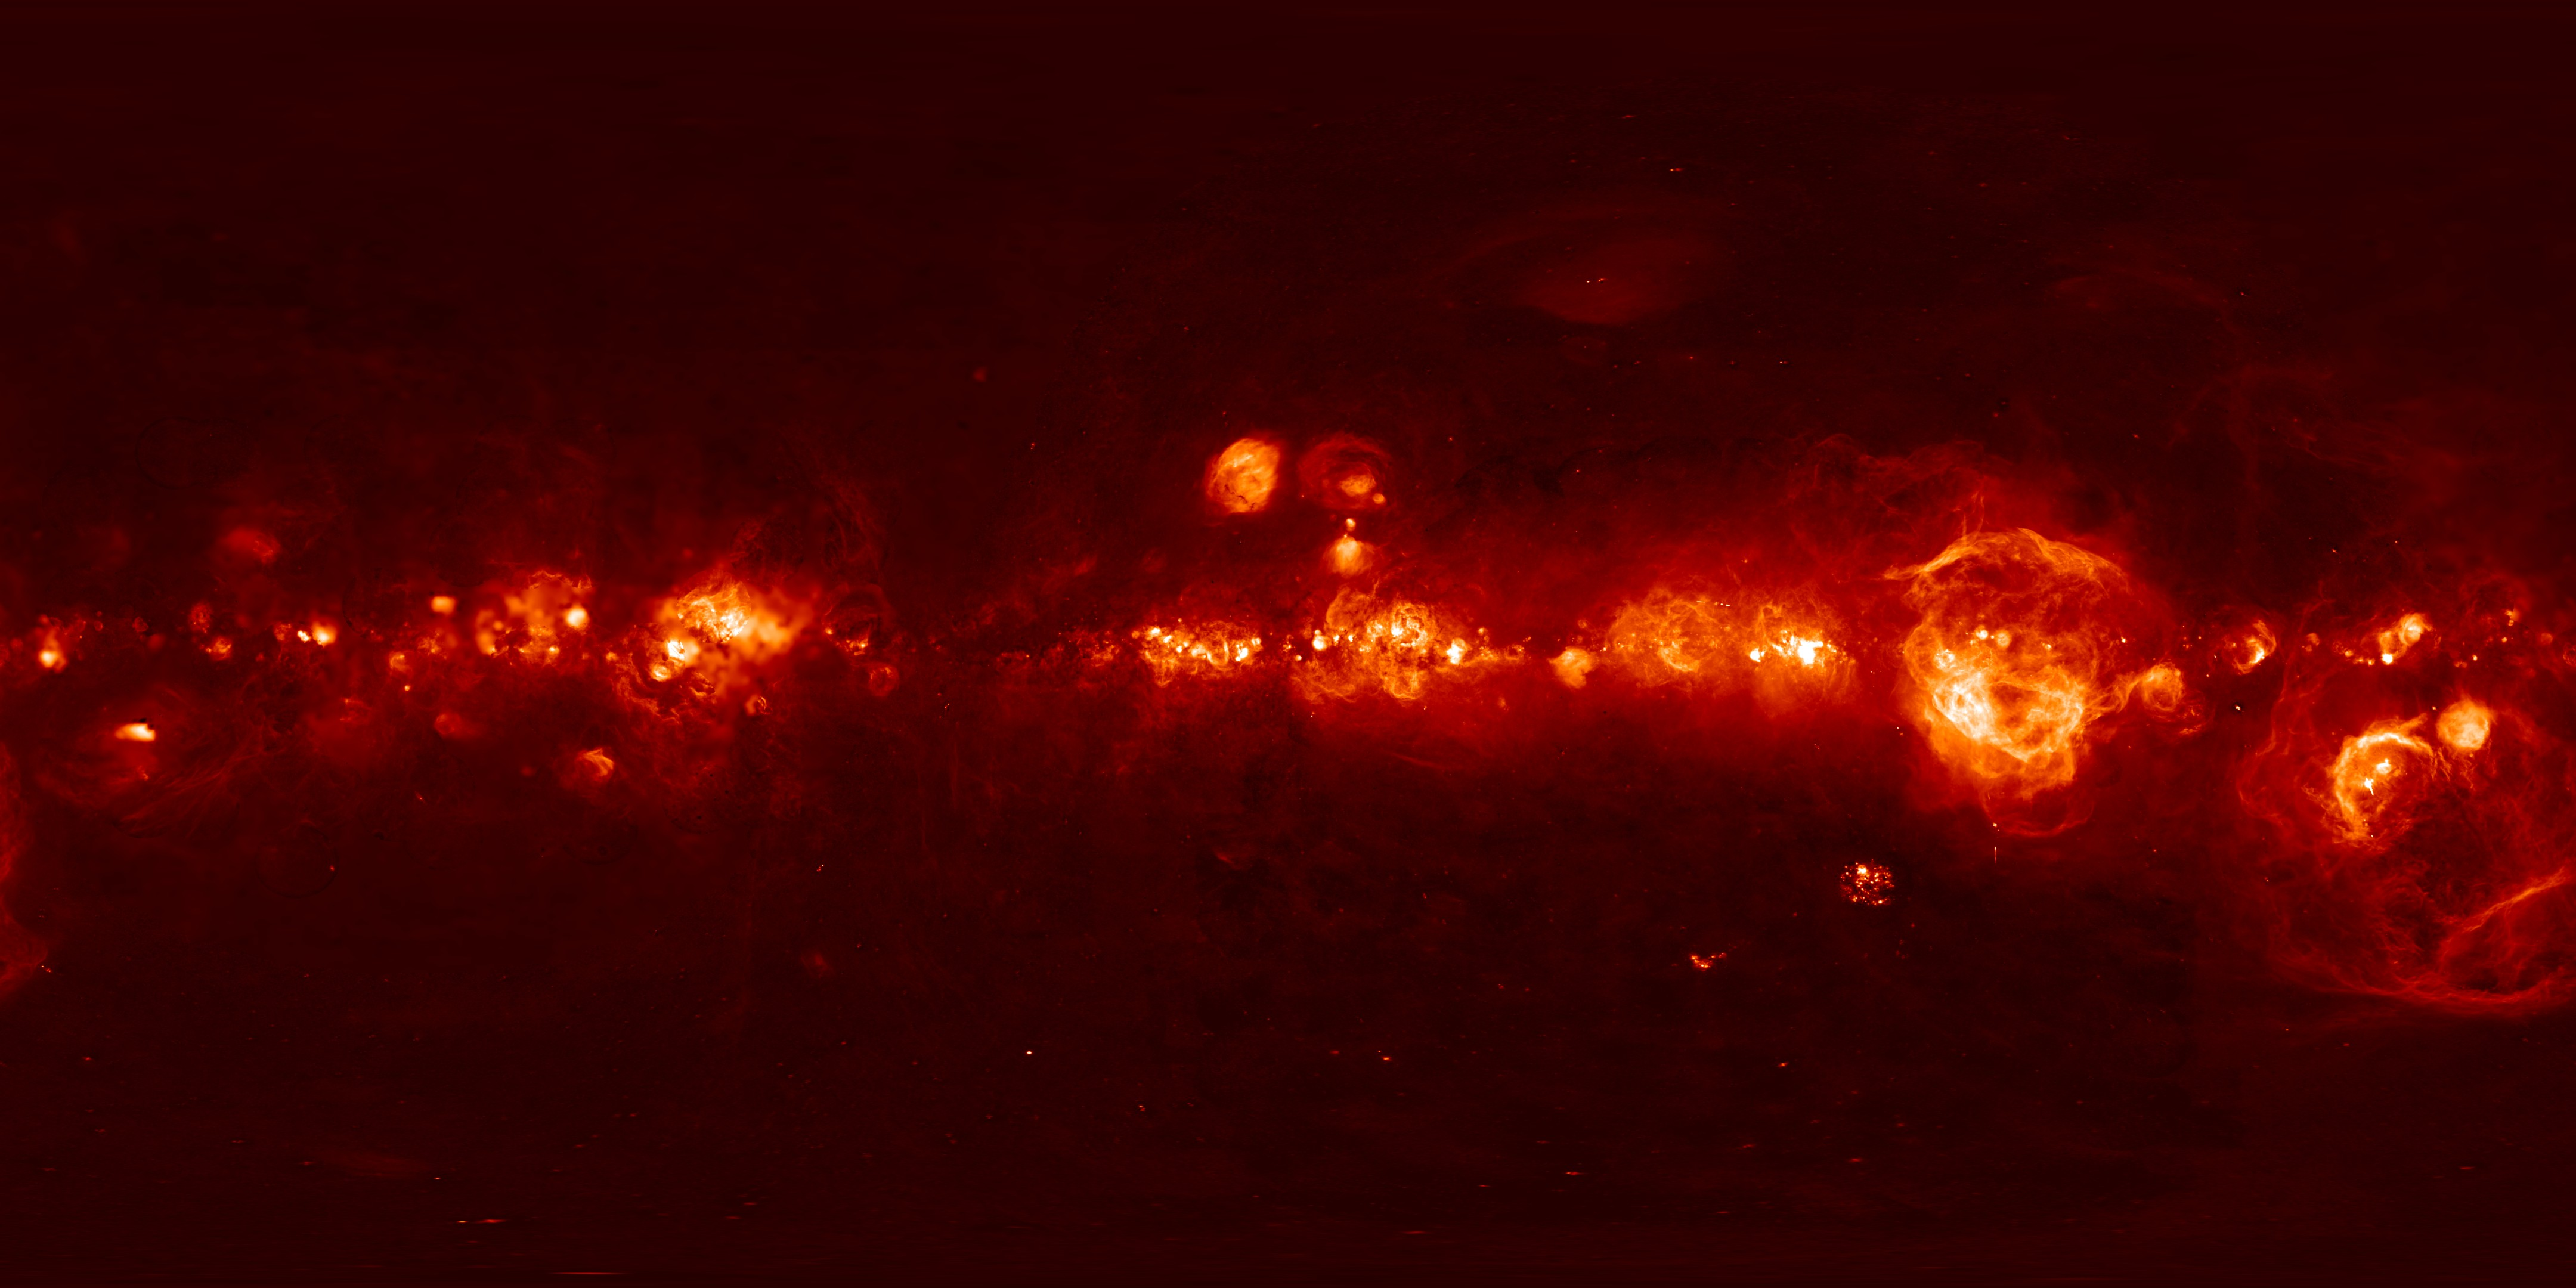
\includegraphics[width=\medpage]{images/Ha.png}
	\caption{Εκπομπή Ha από συνδυασμό τριών διαφορετικών παρατηρήσεων (WHAM - VTSS - SHASSA) Finkbeiner (2003)\cite{finkbeiner_2003}}
\end{figure}

\begin{table}
	\caption{Χαρακτηριστικά της μεσοαστρικής ύλης και περιοχές παρατήρησης}
	\label{tab:ISM}
	\begin{tabular}{p{2.7cm} c  c  c  p{4.75cm}}
		\toprule
		\multirow{2}{*}{Κατηγορία} & Κατάσταση & Θερμοκρασία & Πυκνότητα  & \multirow{2}{*}{Περιοχή Παρατηρήσεων} \\ 
		&  Υδρογόνου & $(K)$ & $(cm^{-1})$ & \\
		\midrule
		Μοριακά Νέφη & Μοριακό \ce{H2} & 10-50 & $>10^3$ & Μοριακή εκπομπή - απορρόφηση στο Ράδιο και στο Υπέρυθρο \\
		Ψυχρά Νέφη \ce{H I} & Ατομικό \ce{H} & $100$ & $30$ & Γραμμή απορρόφησης $21 \,cm$\\
		Θερμό \ce{H I} & Ατομικό \ce{H} & $10^3$ & $0.1$ & Γραμμή εκπομπής $21 \,cm$\\
		Θερμό \ce{H IΙ} & Ιονισμένο \ce{H+} & $10^4$ & $10^{-2}$ & Γραμμή Εκπομπής \ce{H\alpha}\\
		Περιοχές \ce{H IΙ} & Ιονισμένο \ce{H+}& $10^4$ & $>100$ & Γραμμή Εκπομπής \ce{H\alpha}\\
		Υπέρθερμο Ιονισμένο αέριο & Ιονισμένο \ce{H+}& $10^6-10^7$ & $10^{-3}$ & Εκπομπή ακτινοβολίας Χ, Απορρόφηση από ιονισμένα μέταλλα\\
		\bottomrule
	\end{tabular}
\end{table}

%===================================================================
%===================================================================
%===================================================================
	
\section{Μοριακά Νέφη}
Οι πιο ενδιαφέρουσες, από τη σκοπιά της δημιουργίας αστέρων, περιοχές του Μεσοαστρικού Υλικού είναι τα Μοριακά Νέφη (Molecular Clouds).
Τα Μοριακά Νέφη είναι περιοχές όπου ψυχρή μεσοαστρική ύλη έχει πυκνότητες ικανοποιητικά μεγαλύτερες από τη μέση πυκνότητα του μεσοαστρικού υλικού έτσι η ιδιοβαρύτητα του νέφους να παίζει σημαντικό ρόλο στη δυναμική του. 
Αν θέλαμε να υπεραπλουστεύσουμε την όλη διαδικασία της δημιουργίας αστέρων η εικόνα θα ήταν ότι το νέφος καταρρέει και κατακρημνίζεται σε όλο και πιο συμπυκνωμένες δομές έως ότου η πυκνότητα και η μάζα σε μια τέτοια περιοχή είναι αρκετή ώστε να γεννηθούν νέοι αστέρες.   

Όπως φαίνεται και από το όνομα τους, τα Μοριακά Νέφη αποτελούνται κυρίως από μοριακό Υδρογόνο \ce{H2}. Στο γαλαξία μας πάνω από το 80\% του μοριακού Υδρογόνου βρίσκεται σε μοριακά νέφη κατανεμημένα πάνω στις σπείρες του δίσκου αλλά κυρίως σε ένα δακτύλιο ακτίνας 3 με 5 kpc από το κέντρο του γαλαξία \cite{rathborne_2009}.  Από παρατηρήσεις στο \ce{CO} τα μοριακά νέφη δείχνουν να έχουν μάζες που κυμαίνονται από $10^3$ \sm μέχρι και $10^6$ \sm με κατανομή νόμου δύναμης $-1.6$. \cite{stahlern_2004}

Για να δημιουργηθεί το Μοριακό Υδρογόνο καταλυτικό ρόλο παίζει η μεσοαστρική σκόνη.  Όταν δύο άτομα Υδρογόνου ενώνονται και δημιουργούν ένα μόριο \ce{H2} αυτό κερδίζει ενέργεια η οποία όμως δεν μπορεί να αποδοθεί στο περιβάλλον με αποτέλεσμα το μόριο να διασπάται. Παρολαυτά αν η διαδικασία αυτή γίνει πάνω σε έναν κόκκο σκόνης, τότε αυτός λειτουργεί καταλυτικά απορροφώντας το πλεόνασμα ενέργειας και το μόριο παραμένει σταθερό. Έτσι το ουδέτερο Υδρογόνο λειτουργεί σαν καύσιμο που τροφοδοτεί τις πυκνότερες περιοχές του μοριακού Υδρογόνου.

Ένα τυπικό μοριακό νέφος επιβιώνει για $3\times 10^7 \, yr$ πριν καταστραφεί από τους βίαιους αστρικούς ανέμους των αστέρων τύπου O και B που έχουν δημιουργηθεί στο εσωτερικό του. Κατά τη διάρκεια της ζωής του το νέφος αποδίδει τελικά ένα 3\% της μάζας του σε αστέρες. Έτσι για παράδειγμα αν θεωρήσουμε μια τιμή της συνολικής μάζας του μοριακού \ce{H2} στο Γαλαξιακό δίσκο $2\times 10^9$ \sm βρίσκουμε ότι ο ρυθμός δημιουργίας αστέρων (SFR) στο Γαλαξία μας είναι περίπου 2 \sm ανά έτος.  

\subsection{Ενεργειακή ισορροπία στα Μοριακά Νέφη}
Όπως αναφέραμε γενικότερα στη παράγραφο~(\ref{par:EnergyBalance}) η θερμοκρασία ενός νέφους είναι αποτέλεσμα στης ενεργειακής ισορροπίας μεταξύ των μηχανισμών θέρμανσης και ψύξης. Για τα Μοριακά Νέφη συγκεκριμένα η θέρμανση είναι αποτέλεσμα της θερμότητας που παρέχεται από κοντινά άστρα ή μέσω της κοσμικής ακτινοβολίας, ενώ η ψύξη επιτυγχάνεται μέσω διαδικασιών απορρόφησης και κρούσης με τα σωματίδια της σκόνης ή του αερίου.
Η ενέργεια τελικά αποδίδεται μέσω της υπέρυθρης ακτινοβολίας η οποία οφείλεται στην απορρόφηση και την εκπομπή των φωτονίων από το περιβάλλοντα αέριο και σκόνη.

\begin{figure}[h]
	\centering
	\includegraphics[width=15cm]{images/fragmentation.ps}
	\caption{Η ιεραρχική δομή}
\end{figure}

\begin{table}
	\caption{Χαρακτηριστικά και διαφορετικοί τύποι Μοριακών Νεφών}
	\label{tab:MCtypes}
	\begin{tabular}{l c c c c}
		\toprule
		\multirow{2}{*}{Κατηγορία} & Μέση ακτίνα &  Θερμοκρασία & Πυκνότητα \ce{H2} & Μάζα \\ 
		& (pc) & (K) & $(cm^{-3})$ & (\sm) \\
		\midrule
		Γιγαντιαίο Μοριακό Νέφος & $20$ & $15$ & $100$ & $10^5$ \\
		Μοριακό Νέφος & $5$ & $10$ & $300$ & $10^4$\\
		clump & $2$ & $10$ & $10^3$ & $10^3$\\
		Πυρήνας Νέφους & $0.08$ & $10$ & $10^5$ & $10$\\
		\bottomrule
	\end{tabular}
\end{table}

\subsection{Δυναμική και Μορφολογία των Μοριακών Νεφών}

Θεωρούμε ότι το μοριακό νέφος συμπεριφέρεται σαν ένα ιδανικό αέριο με καταστατική εξίσωση
\begin{equation}
P=\frac{k}{\mu m_{H}} \rho T
\end{equation}
όπου $P$ η πίεση, $k$ η σταθερά του Boltzmann, $\mu$ το μέσο μοριακό βάρος, $m_{H}$ η μάζα ενός ατόμου Υδρογόνου, $T$ η θερμοκρασία και $\rho$ η πυκνότητα την οποία σε πρώτη προσέγγιση τη θεωρούμε σταθερή.

Ξεκινώντας με αυτή τη παραδοχή στη συνέχει του κεφαλαίου θα συζητήσουμε τις φυσικές διαδικασίες μέσα στα μοριακά νέφη έως ότου ολοκληρωθεί η δημιουργία αστέρων.

\subsubsection{Εξισώσεις ρευστοδυναμικής}
Το αέριο του μοριακού νέφους δεν είναι στατικό. Η κίνηση μπορεί να περιγραφεί από τις εξισώσεις διατήρησης της μηχανικής ρευστών μέσα σε βαρυτικό πεδίο:
\begin{align}
\text{Εξισωση διατήρησης της Μάζας:  } &\pt{\rho} + \nabla (\rho \vv)=0 \\
\text{Εξισωση διατήρησης της Ορμής:  } &\pt{\vv} +(\vv \cdot \nabla) \vv +\frac{\nabla P}{\rho} -\vec{g}=0
\label{eq:euler}
\end{align}
όπου $\vv=v(x,y,z,t)$ είναι η ταχύτητα του ρευστού σε κάθε σημείο και $\vec{g}=g(x,y,z)$ η επιτάχυνση της βαρύτητας σε κάθε σημείο.
Η τελευταία εξίσωση, η οποία ονομάζεται και εξίσωση Euler, είναι ουσιαστικά ο νόμος του νεύτωνα για ένα συνεχές μέσο.
Έχουμε παραλείψει τους όρους του ιξώδους καθώς στο αραιό μεσοαστρικό χώρο είναι αμελητέοι. Στη ολοκληρωμένη περίπτωση όπου συμπεριλαμβάναμε και τους όρους του ιξώδους τότε θα είχαμε την εξίσωση Navier-Stokes (όπου $\nu$ ο συντελεστής του κινηματικού ιξώδους): 
$$
\pt{\vv} +(\vv \cdot \nabla) \vv +\frac{\nabla P}{\rho} -\vec{g}-\nu \nabla ^2 \vv=0
$$
\textbf{Σε όλες τις παραπάνω εξισώσεις έχουμε κάνει τη παραδοχή ότι η πυκνότητα είναι σταθερή και άρα το ρευστό είναι ασυμπίεστο δηλαδή $\nabla \cdot \vv = 0$.}

Μια δεύτερη παραδοχή που έχουμε κάνει μέχρι αυτό το σημείο είναι ότι οι μοναδικές δυνάμεις που ασκούνται στο υλικό μας είναι οι θερμικές (μέσω της βαθμίδας της πίεσης) και η βαρυτική. Εικάζεται ότι σημαντικό ρόλο στη διαμόρφωση των μοριακών νεφών και τελικά στη κατάρρευση προς τη δημιουργία πρωτοαστέρων παίζει το μεσοαστρικό μαγνητικό πεδίο. Άρα μια ακριβής απεικόνιση της συμπεριφοράς του νέφους θα πρέπει να γίνει μέσω της Μαγνητοϋδροδυναμικής προσέγγισης όπου συμπεριλαμβάνονται οι εξισώσεις του Maxwell και στην εξίσωση της ορμής η δύναμη Lorentz.    

\subsubsection{Βαρυτική αστάθεια}
Μένοντας στη πρώτη προσέγγιση που έχουμε κάνει με ένα άπειρο, ομογενές, στατικό μοριακό νέφος όπου στο κάθε σημείο του ασκούνται δυνάμεις ιδιοβαρύτητας ενώ ταυτόχρονα θεωρούμε ότι η θερμοκρασία του παραμένει κάθε στιγμή σταθερή, άρα $\frac{P}{\rho}=\frac{kT}{\mu m_{H}}=c_s^2=constant$ όπου $c_s$ είναι η ταχύτητα του ήχου για τη θερμοκρασία $T$.

Τώρα θεωρούμε ότι σε κάποια περιοχή του ρευστού έχουμε μια τυχαία τοπική διαταραχή της πυκνότητας όπου γίνεται πυκνότερο κατά $\delta \rho$. Αν θεωρήσουμε επίσης ότι η περιοχή αυτή είναι σφαιρική ακτίνας $r$ τότε θέλουμε να καταλάβουμε το μέγεθος που θα πρέπει να έχει η περιοχή έτσι ώστε η ιδιοβαρύτητα του ρευστού να γίνει αρκετή ώστε να υπερνικήσει την εσωτερική πίεση.

Από την εξίσωση της ορμής \ref{eq:euler} βλέπουμε ότι οι δυνάμεις ανά όγκο εκφρασμένες σαν επιτάχυνση είναι: $\frac{\nabla P}{\rho}$ η δύναμη της εσωτερικής πίεσης και $\vec{g}=-g \hat{r}$ η δύναμη της βαρύτητας θεωρώντας ότι ασκείται ισοτροπικά προς το κέντρο της πυκνότερης περιοχής.
Άρα η κρίσιμη τιμή της ακτίνας θα βρεθεί από την εξίσωση
\begin{equation} 
\label{eq:scaling_gravity}
\frac{\nabla P}{\rho} =-g
\end{equation}
Δεν μας ενδιαφέρει μια ακριβής επίλυση αλλά μια προσέγγιση τάξης μεγέθους της ακτίνας, άρα μπορούμε να προσεγγίσουμε την επιτάχυνση λόγω πίεσης σαν $\frac{\nabla P}{\rho} \sim \frac{P/r}{\rho}=\frac{P}{r \rho}$ ενώ για την επιτάχυνση λόγω βαρύτητας $g=\frac{GM}{r^2}$ όπου $M$ η μάζα που περικλείεται μέσα στη σφαιρική περιοχή, δηλαδή $M \sim r^3 \rho$.

Άρα τελικά, από την (\ref{eq:scaling_gravity}) βρίσκουμε:
\begin{align}
\frac{P}{\rho r} &= \frac{GM}{r^2} \\
\frac{c_s ^2 \rho}{\rho r} &= \frac{Gr^3 \rho}{r^2} \\
r_J&=\frac{c_s}{(G \rho)^{1/2}}
\end{align}
όπου $r_{J}$ είναι η ζητούμενη ακτίνα, η οποία ονομάζεται και ακτίνα Jeans. Αν η περιοχή μας είναι μικρότερη από την ακτίνα αυτή τότε θα από την εξίσωση του νεύτωνα θα έχουμε: 
\begin{equation}
\label{eq:newton}
\ddot{r} \sim \frac{\nabla P}{\rho} -\frac{GM}{r^2} > 0
\end{equation}
άρα η δύναμη λόγω της εσωτερικής πίεσης θα υπερισχύσει και το ρευστό δεν θα καταρρεύσει. Αντίστροφα αν η ακτίνα της συμπύκνωσης είναι μεγαλύτερη από $r_J$ τότε θα καταρρεύσει.

Ισοδύναμα με την ακτίνα Jeans μπορούμε να ορίσουμε την συνολική Μάζα της περιοχής, δηλαδή
\begin{equation}
\boxed{M_J \sim \frac{4}{3} \pi \rho r_J ^3 \sim \frac{4\pi c_s ^3}{3 (G^3 \rho)^{1/2}}}
\end{equation}
Η ταχύτητα του ήχου $c_s$ εξαρτάται μόνο από τη Θερμοκρασία: $c_s \simeq T^1/2$ άρα για τη μάζα Jeans παρατηρούμε ότι:
\begin{equation}
M_J \propto T^{3/2}
\end{equation}

Για τυπικές τιμές ενός μοριακού πυρήνα σε ένα νέφος θερμοκρασίας $10 \, K$ πυκνότητας $10^5 cm^{-3}$ και μέσου μοριακού βάρους $2.3$ (μοριακό Υδρογόνο) βρίσκουμε $r_J=0.05 \,pc$ και $M_J =2$ \sm.

\subsubsection{Κατακρήμνιση}
Αν υποθέσουμε ότι μια περιοχή του μοριακού νέφους με μάζα μεγαλύτερη της μάζας Jeans αρχίζει να καταρρέει ισόθερμα λόγω της ιδιοβαρύτητας της. Η πυκνότητα τότε στο εσωτερικό της θα αρχίσει να αυξάνεται. 

Η μάζα Jeans εξαρτάται από τη πυκνότητα $M_J \propto \rho ^{-1/2}$. Άρα καθώς η πυκνότητα στο εσωτερικό της περιοχής αυξάνεται η μάζα Jeans μικραίνει καθιστώντας  τη βαρυτικά ασταθή. 
Έτσι τυχαίες διαταραχές της πυκνότητας στο εσωτερικό της κάνουν εξαιρετικά πιθανή τη κατάρρευσή της.
Αυτή η διαδικασία επαναλαμβάνεται και στις μικρότερες περιοχές, με τελικό αποτέλεσμα το φαινόμενο της ιεραρχικής κατακρήμνισης.

Η κατακρήμνιση συνεχίζεται έως ότου τα αυτόνομα θραύσματα σταματήσουν να αποκρίνονται ισόθερμα, δηλαδή όσο συνεχίζουν να ακτινοβολούν την ενέργεια που αποκτούν από τη βαρυτική κατάρρευση, οπότε και παραμένουν διαφανή. 
Μόλις φτάσουν στο σημείο να είναι αδιαφανή ή ακτινοβολία παγιδεύεται στο εσωτερικό τους με αποτέλεσμα να θερμαίνονται και έτσι να σταματάει η κατάρρευση.

\subsubsection{Χρόνος ελεύθερης πτώσης}
\label{par:freefall}
Από την εξίσωση~\ref{eq:newton} αν θεωρήσουμε αμελητέα την εσωτερική πίεση \footnote{H προσέγγιση αυτή είναι πολύ λογική αν η κατάρρευση είναι στα αρχικά της στάδια} τότε η εξίσωση του νεύτωνα γίνεται:
\begin{equation}
\ddot{r}=-\frac{GM}{r^2}
\end{equation}
Κάνοντας ανάλυση κλίμακας όπως προηγουμένως, βρίσκουμε τη χαρακτηριστική χρονική κλίμακα κατάρρευσης:
\begin{equation}
t_{ff}\simeq \left(\frac{R^3}{GM}\right)^{1/2} \simeq \left( \frac{1}{G \rho}\right) ^(1/2) \simeq \frac{r_j}{c_s} 
\end{equation}
Η ακριβής επίλυση της εξίσωσης αν "ξεφορτωθούμε" και τη κλίμακα μήκους $R$ μέσω της σχέσης $M/R^3 \simeq \rho$ μας δίνει αποτέλεσμα:
\begin{equation}
t_{ff}=\left( \frac{3 \pi}{32 G \rho}\right) ^{1/2} \sim 2.1\times 10^3 \rho ^{-1/2} \, s
\end{equation}
Για ένα μοριακό νέφος αρχικής πυκνότητας $10^{-13}\, g\,cm^{-3}$ ο χρόνος αυτός είναι $\sim 2\times 10^5 \, yr$. Ο χρόνος αυτός είναι μικρότερος από τη μέση παρατηρούμενη ηλικία των μοριακών νεφών $(\sim 10^7\ yr$ \ref{par:MCtc}). Οπότε είναι προφανές ότι πέρα απο τη βαρύτητα υπάρχουν και άλλοι μηχανισμοί που επηρρεάζουν τη κατάρρευση.


\subsubsection{Θεώρημα Virial}
Η μέχρι στιγμής ανάλυση μας βασίζεται σε αρκετές συμβάσεις και προσεγγίσεις που μας δίνουν μια πολύ γενική και εξιδανικευμένη εικόνα.
Μια καλύτερη μέθοδος για να εξετάσουμε τη δυναμική ενός απομονωμένου νέφους είναι να εφαρμόσουμε το θεώρημα Virial, δηλαδή την εξίσωση της ενέργειας.
Το θεώρημα Virial προκύπτει από τη διαφόριση της ροπής αδράνειας του νέφους, όπου η ροπή αδράνειας ορίζεται ως: 
\begin{equation}
I=\int \rho |\vec{r}|^2 \, dV
\end{equation}
Η εξίσωση της ενέργειας παράγεται από τη δεύτερη χρονική παράγωγο της ροπής αδράνειας η οποία μας οδηγεί στη:
\begin{equation}
\frac{1}{2}\ddot{I}=2\TT+2\UU +\WW+\MM -3P_{surf}V
\end{equation}
όπου $\TT$ η ολική κινητική ενέργεια λόγω της κίνησης του νέφους στην οποία συμπεριλαμβάνεται η τύρβη και η περιστροφή του νέφους:
\begin{equation}
\TT = \frac{1}{2} \int \rho |\vec{u}|^2 dV
\end{equation}
$\UU$ η εσωτερική ενέργεια λόγω θερμικών κινήσεων:
\begin{equation}
\UU=\frac{3}{2} \int n k_B T dV=\frac{3}{2} \int P dV
\end{equation}
$\WW$ η βαρυτική δυναμική ενέργεια αν $\Phi _g$ το βαρυτικό δυναμικό:
\begin{equation}
\WW=\frac{1}{2} \int \rho \Phi _g dV
\end{equation}
$\MM$ η ενέργεια του μαγνητικού πεδίου:
\begin{equation}
\MM=\frac{1}{8\pi} \int |\vec{B}|^2 dV
\end{equation}
$V$ ο όγκος του νέφους και $P_{surf}$ η εξωτερική πίεση. 
\subsubsection{Ημιστατική κατάσταση}
Στη κατάσταση ισορροπίας το θεώρημα Virial γράφεται:
\begin{equation}
\label{eq:Virial}
2\TT+2\UU +\WW+\MM -3P_{surf}V=0
\end{equation}
Μπορούμε να απλοποιήσουμε τις παραπάνω σχέσεις παίρνοντας τον μέσο μέσα σε έναν όγκο ελέγχου. Έτσι για το κάθε όρο βρίσκουμε:
\begin{align}
\TT &= \TT_{turbulence}+\TT_{rotation} = \frac{1}{2} M \Delta u_{turb} ^2 + C_{rot} M R^2 \Omega ^2\\
\UU &= \frac{3}{2} P V=\frac{3}{2} c_s ^2 \rho V=\frac{3}{2} M c_s ^2 \\
\WW &= -C_{grav} \frac{GM^2}{R} \\
\MM & = C_{mag}\frac{\Phi^2}{3 \pi ^2 R}
\end{align}
\noindent

%\begin{table}
\begin{tabular}{|c p{9cm}}
$P,\rho$ &οι \textbf{μέσες τιμές} της πίεσης και της πυκνότητας \\
$M$ &η μάζα που εσωκλείεται στον όγκο ελέγχου\\
$c_s =\left( \frac{k_B T}{\mu m_H}\right) ^{1/2}$ &η ταχύτητα θερμικών κινήσεων των μορίων \\
$\Delta u$ &η διασπορά της ταχύτητας λόγω τυρβώδους κίνησης \\
$\Omega$ &η γωνιακή ταχύτητα του νέφους που τη θεωρούμε τοπικά ομογενή \\
$\Phi=\pi R^2 B$ &η ροή του μαγνητικού πεδίου \footnote{Χρησιμοποιούμε τη ροή του μαγνητικού πεδίου γιατί } \\
$C_{rot}$ &παράμετρος που αφορά τη κατανομή της μάζας, στην ομογενή περίπτωση ισούται με $\frac{1}{5}$ \\
$C_{grav}$ &παράμετρος που αφορά τη κατανομή της μάζας, στην ομογενή περίπτωση ισούται με $\frac{3}{5}$ \\
$C_{mag}$ &παράμετρος που αφορά το σχήμα του νέφους και τη τοπολογία του μαγνητικού πεδίου, για σφαίρα $\frac{3}{4}$ ενώ για δίσκο $\frac{1}{\pi}$
\end{tabular}
%\end{table}

\medskip

Ορίζουμε σαν διασπορά ταχύτητας $\sigma ^2$ σε μια διεύθυνση το άθροισμα της διασποράς λόγω θερμικών κινήσεων $c_s ^2 $ και της τυρβώδους ροής $\Delta u _i $, δηλαδή:
\begin{equation}
\label{eq:dispersion}
\sigma ^2=\frac{k_B T}{\mu \, m_H}+ \Delta u^2
\end{equation} 

\subsubsection{Μάζα Virial}
\label{par:VirialMass}
Για ένα σφαιρικό απομονωμένο νέφος μάζας $M$, ακτίνας $R$ με διασπορά ταχύτητας $\sigma$ (\ref{eq:dispersion}), αγνοώντας τις επιδράσεις του μαγνητικού πεδίου και της περιστροφής από τη σχέση~\ref{eq:Virial} για την ισορροπία βρίσκουμε:
\begin{align}
\WW &\simeq M\sigma ^2 \\
M_{virial} &\sim \frac{\sigma ^2 R}{G} 
\end{align} 
Άν η μάζα του νέφους ξεπερνάει τη μάζα Virial τότε το νέφος δεν βρίσκεται σε ισορροπία και θα καταρρεύσει αν δεν συγκρατηθεί από κάποιον άλλο μηχανισμό.

Στο θεώρημα Virial η μόνη αρνητική επίδραση είναι αυτή της βαρύτητας. Είναι η μόνη δύναμη που συνεισφέρει στη συμπύκνωση του νέφους σε αντιπαράθεση με τη θερμική κίνηση των μορίων, τη τύρβη, το μαγνητικό πεδίο και τη περιστροφή του νέφους.

Χωρίς να επεκταθούμε παραπάνω, μπορούμε να εργαστούμε αναλόγως με τη μάζα Virial ώστε να υπολογίσουμε τη κρίσιμη μάζα του νέφους σε μια σειρά σεναρίων όπου θα λαμβάνονταν υπόψη και οι επιδράσεις της περιστροφής, του μαγνητικού πεδίου κλπ.

Η περιστροφή αν και λόγω της μικρής αρχικής γωνιακής ταχύτητας του νέφους $(\Omega \sim 10^{-14} s^{-1})$ μπορεί να παίξει σημαντικό ρόλο καθώς αυξάνεται σε μεγάλο βαθμό κατά τη κατάρρευση \footnote{στη κατάρρευση του νέφους η ακτίνα του μειώνεται κατά έναν παράγοντα $10^7$ άρα από τη διατήρηση της στροφορμής $\Omega R^2 = const.$ βρίσκουμε η γωνιακή του ταχύτητα αυξάνεται κατά παράγοντα $10^{14}$}. Οι παρατηρήσεις μας δείχνουν ότι η στροφορμή είναι αρκετά μικρότερη από την αναμενόμενη, κάτι που μάλλον οφείλεται στο φαινόμενο του "μαγνητικού φρεναρίσματος", δηλαδή την επιβράδυνση της περιστροφής του μοριακού πυρήνα - πρωτοαστέρα λόγω της μεταφοράς στροφορμής μέσω κυμάτων Alfven στις μαγνητικές γραμμές.

Για λόγους πληρότητας θα παραθέσουμε τις αντίστοιχες μάζες \cite{schulz_2012} Virial για ένα νέφος όπου η μαγνητική πίεση μαγνητικού πεδίου έντασης $B$ ισορροπεί τη βαρύτητα:
\begin{equation}
M_{\phi} \sim 3.5 \times \frac{B^3}{G^{3/2} \rho^2} 
\end{equation}
και για νέφος όπου η στροφορμή $J$ ισορροπεί τη βαρύτητα:
\begin{align}
M_{rot} = 5.1 \left( \frac{\sigma J}{G M} \right) 
\end{align}

\subsubsection{Σχέσεις του Larson}
\label{par:LarsonLaws}
Οι θερμικές τυχαίες κινήσεις ενός μορίου μαζί με τις τυχαίες ταχύτητες της τύρβης συνιστούν αυτό που ορίσαμε και προηγουμένως διασπορά της ταχύτητας $\sigma$. Αν από ένα νέφος αερίου παρατηρήσουμε μια γραμμή εκπομπής τότε λόγω της διασποράς το προφίλ της γραμμής θα "διογκωθεί" λόγω του φαινομένου Doppler. 

Ένα χρήσιμο μέγεθος για τη παραμετροποίηση μια γραμμής εκπομπής είναι το πάχος της στο ύψος που αντιστοιχεί στο μισό της μέγιστης έντασης (Full Width at Half Maximum - FWHM). Εφόσον η γραμμή εκπομπής αντιστοιχεί σε μια κατανομή gauss τότε το πάχος αυτό είναι: $\Delta u _{FWHM = }\sqrt{8 \ln(2)} \sigma _{SD}$, όπου $\sigma _{SD}$ η τυπική απόκλιση της κατανομής. 

Κινούμενοι αντίστροφα από το φαινόμενο Doppler μπορούμε να μεταφέρουμε τη καμπύλη των συχνοτήτων στο χώρο των ταχυτήτων. Μετρώντας λοιπόν τη τιμή FWHM στο χώρο των ταχυτήτων έχουμε μια καλή προσέγγιση για την τιμή της διασποράς της ταχύτητας $\sigma$.

To 1981 ο Larson \cite{larson_1981} μετρώντας τη ταχύτητα διασποράς στις γραμμές εκπομπής \ce{CO}, \ce{H2CO}, \ce{NH3} κ.α. διαφορετικών μοριακών νεφών κατέγραψε κάποιες εμπειρικές σχέσεις η οποίες και ονομάζονται σχέσεις του Larson (Larson Laws). Στη συνέχεια παραθέτουμε τις αντίστοιχες σχέσεις από τους Solomon et al. (1987) \cite{solomon_1987} καθώς αφορούν περισσότερα δεδομένα.
Η πρώτη σχέση συνδέει τη διασπορά με το μέγεθος του νέφους:
\begin{equation}
\label{eq:LarsonR}
\sigma \simeq (0.72 \pm 0.07)\, R^{(0.5 \pm 0.2)} \ km\, s^{-1}
\end{equation} 
\todo{fwto larson R-s law}
Αν η διασπορά της ταχύτητας ήταν λόγω μόνο των θερμικών κινήσεων τότε αυτή θα εξαρτιόταν μόνο από τη θερμοκρασία που όμως για τις παρατηρήσεις είναι σταθερή με τιμή περίπου στους $10 \ K$. Η θερμική ταχύτητα γι αυτή τη θερμοκρασία είναι $0.19\ km\, s^{-1}$.
Άρα είναι εμφανές ότι η τύρβη παίζει πολύ σημαντικό ρόλο στη δυναμική των μοριακών νεφών. Ένα δεύτερο συμπέρασμα που μπορούμε να βγάλουμε είναι ότι για μεγέθη μεγαλύτερα των $0.1 \ pc$ η τύρβη είναι υπερηχητική.

Η δεύτερη σχέση συνδέει τη μάζα του νέφους με τη διασπορά:
\begin{equation}
\label{eq:LarsonM}
\sigma = 0.15\, M^{0.25}
\end{equation}
\todo{fwto larson M-s law}
Από τη σχέση αυτή μπορούμε να βρούμε τη σχέση μάζας-ακτίνας:
\begin{equation}
M\propto R^2
\end{equation}
και εφόσον $\rho = M/R^3$
\begin{equation}
\label{eq:Larsonrho}
\rho \propto R^{-1}
\end{equation}
το οποίο συμπίπτει και με παρατηρησιακά δεδομένα $(\rho \propto R^{-1.1})$.
\todo{fwto larson M-rho law}
\medskip

Από τις σχέσεις (\ref{eq:LarsonM}) και (\ref{eq:LarsonR}) μπορούμε να συγκρίνουμε τα πειραματικά αποτελέσματα με τη προσέγγιση Virial~\ref{par:VirialMass}: 
$$
\frac{M}{R \sigma ^2}\sim \frac{1}{G}
$$
άρα θα έχουμε
\begin{equation}
\frac{M}{R}\propto \sigma ^2 \rightarrow \frac{M}{R \sigma ^2}=const.
\end{equation}
δηλαδή φαίνεται η προσέγγιση Virial που κάναμε να είναι αρκετά ικανοποιητική, ενώ αποδεικνύεται ότι εν τέλει η υπερηχητική τύρβη να είναι υπεύθυνη τελικά για την εξισορρόπησης τη βαρύτητας σε νέφη μεγάλης μάζας. 

\subsection{Τύρβη στα μοριακά νέφη}
Η τύρβη είναι μια ιδιότητα της ροής των φυσικών ρευστών που οφείλεται στη μη-γραμμικότητα της μεταφοράς ορμής η οποία επιτρέπει την αλληλεπίδραση δομών της ροής σε διαφορετικές χωρικές κλίμακες, με επακόλουθο μια διαταραχή συγκεκριμένης χαρακτηριστικής χωρικής κλίμακας να εξαπλώνεται σε προοδευτικά μεγαλύτερες και μικρότερες κλίμακες \cite{sofianos_turbulence}.

Μια διαταραχή συγκεκριμένης χωρικής κλίμακας, που δημιουργείται λόγω εισροής ενέργειας, διασπάται κυρίως σε μικρότερης κλίμακας διαταραχές μέχρι ένα χαρακτηριστικό όριο. Το όριο αυτό που ονομάζεται Kolmogorov microscale είναι και το σημείο όπου τελικά η κινητική ενέργεια μετατρέπεται σε θερμική μέσω της μοριακής διάχυσης. Για ένα μοριακό νέφος το όριο Kolmogorov microscale είναι της τάξης $10^{-5} pc$.

Η διαδικασίας αυτή δημιουργεί μια κατανομή κατακρήμνισης διαταραχών γνωστή σαν νόμο Kolmogorov-Obhukov, η οποία εκφρασμένη για τη ταχύτητα διασποράς γράφεται σαν:
\begin{equation}
\sigma \propto L^{1/3}
\end{equation} 
όπου $L$ η χαρακτηριστική κλίμακα της διαταραχής.

Σε ένα μοριακό νέφος οι "πηγές" μιας τέτοιας ενέργειας εισόδου μπορεί να είναι:
\begin{itemize}
	\item η διάτμηση λόγω της διαφορικής περιστροφής του γαλαξιάκου δίσκου,
	\item εκροές ύλης από πρωτοαστέρες μέσα στο νέφος,
	\item αστρικοί άνεμοι και
	\item εκρήξεις supernova
\end{itemize}

Όπως είδαμε από τις παρατηρήσεις, στα μοριακά νέφη η σχέση που συνδέει τις ταχύτητες διασποράς με τη κλίμακα ακολουθεί ένα νόμο δύναμης με κλίση $0.5 \pm 0.2$.  Ο λόγος που διαφέρει με τον νόμο δύναμης Kolmogorov-Obhukov (κλίση $0.3$) μάλλον οφείλεται στο ότι η τυρβώδης κίνηση στα μοριακά νέφη είναι ισχυρά υπερηχητική (αριθμός Mach > 10).
Αυτό δεν συνάδει με τις υπάρχουσες θεωρίες τύρβης που έχουμε σήμερα, ενώ η διαδικασία διάχυσης δεν συμβαίνει απαραίτητα στις χαμηλές κλίμακες λόγω των κυμάτων κρούσης των υπερηχητικών ροών που παράγουν θερμότητα.

\subsubsection{Διάσταση Fractal}
Η τύρβη επίσης προβλέπει και την fractal δομή των μοριακών νεφών, δηλαδή τη ομοιότητα της δομής τους ανεξαρτήτως της κλίμακας που παρατηρούμε. 
Η δομή Fractal χαρακτηρίζεται από μια παράμετρο που ονομάζεται διάσταση fractal, η οποία συνδέει τη περίμετρο $P$ μια κλειστής καμπύλης (π.χ. μια ισοϋψής της πυκνότητας ενός νέφους) με το εμβαδόν $A$ της καμπύλης μέσω της σχέσης:
\begin{equation}
P\propto A^{D/2}
\end{equation}
Η μέτρηση της παραμέτρου γίνεται με τη χρήση διαφόρων αλγορίθμων, όπως του αλγορίθμου Box Counting ($D_B$) όπου το αντικείμενο καλύπτεται με μια σειρά τετραγώνων μήκους $\epsilon$. Η διάσταση βρίσκεται από τη σχέση:
\begin{equation}
D_B = \lim_{\epsilon \to 0} \frac{\log N(\epsilon)}{\log (1/\epsilon)}
\end{equation}
όπου $N(\epsilon)$ είναι ο αριθμός των τετραγώνων διάστασης $\epsilon$ που χρειάζονται για να καλύψουν το χώρο. Όσο το $\epsilon \to  0$ το $N(\epsilon)$ αυξάνεται μέσω της σχέσης:
\begin{equation}
N(\epsilon) \propto \epsilon ^{-D_B}
\end{equation}
άρα με μια μέθοδο ελαχίστων τετραγώνων των τιμών $\left(\log N(\epsilon),\log \epsilon\right)$ βρίσκουμε τη τιμή $D_B$.

\textbf{Παρατηρήσεις στα μοριακά νέφη δίνουν τιμές της διάστασης fractal παρόμοιες με τυρβώδεις εργαστηριακές ροές αλλά και γήινων ατμοσφαιρικών νεφών δηλαδή $D\sim 1.35$}
 
 %Η ιεραρχική κατακρήμνιση είναι εμφανής στα μοριακά νέφη όπως  φαίνεται και από το πίνακα~\ref{tab:MCtypes}. Η δομή αυτή 
 %Η παραπάνω διαδικασία δίνει στα μοριακά νέφη μια ιεραρχικά δομημένη μορφή όπου οι πυκνότερες περιοχές έχουν μικρότερη κλίμακα μήκους (clumpiness). Εκτός όμως από τη clumpiness \todo{διατύπωση} μορφολογία, που, παρατηρούμε και νηματώδεις (filaments) δομές συμπυκνώσεων.
 
 
 %\subsubsection{Φωτο-διάσπαση}
 %Για να "επιβιώσει" ένα μοριακό νέφος τα μόρια θα πρέπει να προστατευτούν από τη διάσπαση λόγο φωτονίων ενέργειας μεγαλύτερης των \SI{13.6}{\electronvolt} με μήκος κύματος μικρότερο από \SI{912}{\angstrom} . Τέτοια φωτόνια, που ανήκουν στο φάσμα του extreme \todo{μεταφραση} υπεριώδους (EUV) δημιουργούνται κυρίως από αστέρες O και B αλλά είναι πολύ δύσκολο να φτάσουν στα μόρια καθώς ιονίζουν το ατομικό υδρογόνο το οποίο με τη σειρά του εκπέμπει φωτόνια μεγαλύτερου όμως μήκους κύματος.
 

\subsection{Χρόνος ζωής των μοριακών νεφών}
\label{par:MCtc)}
Είδαμε στη παράγραφο (\ref{par:freefall}) ότι ο χρόνος κατάρρευσης ενός μοριακού νέφους είναι της τάξης των $10^5 \ yr$. Αυτή η τιμή είναι μια κατώτερη τιμή της ηλικίας ενός νέφους καθώς χωρίς τους υποστηρικτικούς μηχανισμούς το νέφος θα καταστραφεί δημιουργώντας αστέρες.

Μια συντηρητική ανώτερη τιμή της χρονικής κλίμακας της ζωής ενός μοριακού νέφους μπορεί να παραχθεί μέσω του θεωρήματος Virial για τη διασποράς της ταχύτητας. Υπό την απουσία εξωτερικής πίεσης και αγνοώντας το όποιο μαγνητικό πεδίο και άλλους μηχανισμούς ανάδρασης, ένα μοριακό νέφος με χαρακτηριστική διασπορά ταχύτητας $\sigma \sim 10 \ km \, s^{-1}$ και ακτίνας $R \sim 100 \ pc$ θα διαλυθεί μέσα σε χρόνο:
\begin{equation}
t_{disp} \simeq \frac{R}{\sigma} \simeq 10^7 \ yr
\end{equation} 

Τέλος, μπορούμε να βρούμε και μια τρίτη τιμή της ηλικίας των μοριακών νεφών μέσω της φωτο-διάσπασης και φωτο-εξάτμισης των μορίων από την ακτινοβολία υψηλών ενεργειών \footnote{πρόκειται για φωτόνια με ενέργεια μεγαλύτερη των $5 \ eV$ στο Υπεριώδες και X μέρος τους φάσματος} αστέρων τύπου O και B που έχουν γεννηθεί στο εσωτερικό του μοριακού νέφους. Ένας τέτοιος αστέρας μπορεί να ιονίζει το περιβάλλον του για ένα διάστημα $10^6 \ yr$ με ρυθμό $3-5 \times 10^{-3} \ M_{\odot} \, yr^{-1}$ δίνοντας σε ένα μοριακό νέφος χρόνο ζωής τάξης $10^7 \ yr$ ώσπου να καταστραφεί από μερικές γενιές τέτοιων αστέρων.

Από παρατηρήσεις ανοιχτών νεαρών αστρικών σμηνών, όπως για παράδειγμα οι πλειάδες, τα μοριακά νέφη παρατηρούνται να έχουν ηλικίες της τάξης των $10^7 yr$ \cite{bash_1977}, \cite{leisawitz_1989}.
Αυτό υποδηλώνει ότι τουλάχιστον οι μηχανισμοί ανάδρασης και η τύρβη έχουν κυρίαρχο ρόλο στο κύκλο ζωής ενός μοριακού νέφους.

\subsection{Κατανομή μαζών των μοριακών πυρήνων} 
Όπως είπαμε και στην εισαγωγή, παρατηρήσεις στο \ce{CO} σε διαφορετικά μοριακά νέφη, και σε διαφορετικές κλίμακες (μοριακά νέφη, clumps και πυρήνες) η κατανομή των μαζών φαίνεται να είναι της μορφής:
\begin{equation}
\frac{dN}{dM} \propto M^{-x}
\end{equation}
όπου $dN$ είναι ο αριθμός των νεφών με μάζες από $M$ μέχρι $M+dM$ με άνω όριο περίπου τις $10^6$ \sm. Για τα clumps η λογαριθμική κλίση είναι από $1.6$ μέχρι $1.8$.\todo{φωτο mass clump spectrum}

Αυτή η κατανομή είναι πολύ πλατύτερη της αντίστοιχης κατανομής μαζών των αστέρων της κύριας ακολουθίας βλέπε παρακάτω (\ref{par:imf}). Αυτό μπορεί να εξηγηθεί εφόσον ένα clump είναι μια περιοχή που δεν συνδέεται τόσο άμεσα με τη δημιουργία αστέρων, καθώς υπάρχουν clumps που δεν θα δημιουργήσουν απαραίτητα αστέρες ή αστρικά σμήνη, ακόμα και clumps που μπορεί να μην είναι καν βαρυτικά συνδεδεμένα (gravitionally bound).

Παρόλαυτα αυτό δεν συμβαίνει και με τους μοριακούς πυρηνές, όπως θα αναφέρουμε στη συνέχεια. 

\subsubsection{Initial Mass Function}
\label{par:imf}
Η Initial Mass Function (IMF) είναι μια εμπειρική συνάρτηση που χαρακτηρίζει τη κατανομή των αστρικών μαζών στην αρχή της ζωής τους \footnote{δηλαδή μόλις μπούν στη Κύρια Ακολουθία} για ένα συγκεκριμένο πληθυσμό αστέρων. Η IMF παρουσιάζει ίδια μορφή με μικρές σχετικά αποκλίσεις μεταξύ διαφορετικών πληθυσμών αστέρων. \cite{salpeter_initial_2005}
Πέρα από τη κατανόηση της σημασίας της παγκοσμιότητας της, η IMF είναι πάρα πολύ σημαντικό εργαλείο καθώς τα χαρακτηριστικά και η εξέλιξη ενός αστέρα εξαρτώνται από τη μάζα του. 
Άρα η καλύτερη δυνατή προσέγγιση της IMF βρίσκεται στο κέντρο της έρευνας για την εξέλιξη αστρικών πληθυσμών και γαλαξιών.

\paragraph{Μορφή της IMF}
Η IMF συνήθως \footnote{Πέρα από τη μορφή νόμου δύναμης, η IMF μπορεί να οριστεί και σαν λογαριθμική κανονική κατανομή \cite{salpeter_initial_2005}} ορίζεται σαν μια σειρά διαδοχικών νόμων δύναμης της μορφής 
\begin{equation}
\frac{dN}{dm} \propto m^{-\alpha}
\end{equation}

Ο Salpeter (1955) ήταν ο πρώτος που ασχολήθηκε με το συγκεκριμένο πρόβλημα υπολόγισε από παρατηρησιακά δεδομένα τη παράμετρο $\alpha=2.35$.
Ο Kroupa (2001) χώρισε την IMF σε τρείς νόμους δύναμης με διαφορετικό εκθέτη:

\begin{align}
\alpha&=0.3 \pm 0.7 \text{ για μάζες απο $0.01$\sm έως $0.08$\sm} \\
\alpha&=1.3 \pm 0.5 \text{ για μάζες απο $0.08$\sm έως $0.5$\sm} \\
\alpha&=2.3 \pm 0.3 \text{ για μάζες πάνω απο $0.5$\sm}
\end{align}

\subsubsection{IMF και δημιουργία αστέρων}
Είναι προφανές το ενδιαφέρον του ερευνητικού κλάδου της δημιουργίας αστέρων για την IMF καθώς κάθε θεωρία δημιουργίας αστέρων θα πρέπει να είναι ικανή να εξηγεί και τη "παγκόσμια" μορφή της IMF.
Έτσι μέσω παρατηρήσεων των πυκνών πυρήνων στα μοριακά νέφη, βρήκαμε ότι η κατανομή των μαζών τους (Dense Core Mass Function - DCMF) μοιάζει με αυτή των αστέρων της κύριας ακολουθίας με τη διαφορά ότι είναι μετατοπισμένη κατά ένα παράγοντα $3$ προς τις μεγαλύτερες μάζες, με το σημείο αλλαγής της κλίσης να είναι στις $2-3$ \sm σε σχέση με τις $0.5$ \sm της IMF. 

Αν και θα πρέπει να είμαστε ιδιαίτερα προσεκτικοί με τις συγκρίσεις των δύο κατανομών, καθώς υπάρχουν μεγάλες απροσδιοριστίες στα άνω και κάτω όρια της DCMF \cite{polychroni__2010}, το συμπέρασμα που βγάζουμε με τα μέχρι τώρα αποτελέσματα, είναι ότι μηχανισμοί ανάδρασης όπως οι εκροές μάζας (outflows) και οι αστρικοί άνεμοι από τους πρωτοαστέρες εμποδίζουν τη περαιτέρω κατάρρευση του πυρήνα και με τη πάροδο του χρόνου τον διαλύουν. Έτσι μπορούμε να κάνουμε μια εκτίμηση για την απόδοση των πυκνών πυρήνων που δεν ξεπερνά το 30\%.

\section{Παρατηρήσεις των Μοριακών Νεφών}
\label{par:H2}
Παρά τη "κυριαρχία" του μοριακού υδρογόνου στα Μοριακά Νέφη είναι απίθανο να το παρατηρήσουμε καθώς η ενεργειακή διαφορά ακόμα και των χαμηλότερα διεγερμένων από τη βασική του στάθμη είναι πολύ μεγάλη, όπως θα δείξουμε παρακάτω. Έτσι στις χαμηλές θερμοκρασίες των Μοριακών Νεφών, η μόνη δυνατότητα να παρατηρήσουμε άμεσα το \ce{H2} είναι μέσω γραμμών απορρόφησης από πηγές στο υπόβαθρο. \footnote{μέσω των γραμμών απορρόφησης στο Υπεριώδες} 

Ο εναλλακτικός τρόπος παρατήρησης του \ce{H2} είναι εμμέσως μέσω της εκπομπής διαφορετικών μορίων που είναι πιο "ευαίσθητα" στις χαμηλές θερμοκρασίες, όπως του Μονοξειδίου του Άνθρακα (\ce{^{12}CO}) και των ισοτόπων του (\ce{^{13}CO}, \ce{C^{18}O}), της αμμωνίας (\ce{NH3}) και άλλων (\ce{CS}, \ce{H2CO}, \ce{H2O}, \ce{OH}).
Γνωρίζοντας την αναλογία μεταξύ των μορίων μπορούμε να υπολογίσουμε τη ποσότητα του \ce{H2}.

Εκτός από την παρατήρηση της μοριακής συνιστώσας του νέφους, έχουμε στη διάθεση μας και άλλες περιοχές παρατήρησης όπως η εκπομπή των κόκκων σκόνης στο Υπέρυθρο και η εξάλειψη από τους ίδιους του ορατού φώτος αστέρων του υποβάθρου.

\subsection{Ενεργειακές μεταβάσεις του \ce{H2}}
Το \ce{H2} είναι ένα πλήρως συμμετρικό μόριο επομένως δεν έχει μόνιμη διπολική ροπή. Άρα καθώς οι μεταβάσεις του ηλεκτρικού διπόλου είναι απαγορευμένες οι επόμενες είναι οι τετραπολικές. 
Η ενέργεια περιστροφής είναι $E_{rot}=\frac{h^2}{2I_{H_2}}J(J+1)$ όπου $J$ ο περιστροφικός κβαντικός αριθμός και $I_{H_2}=5\times 10^{-48} \, kg\, m^2$ η ροπή αδράνειας του \ce{H2}.
Για τις τετραπολικές μεταβάσεις έχουμε ότι $\Delta J =0,\pm 2$, άρα για το \ce{H2} αυτό μπορεί να βρίσκεται σε δύο μορφές, αυτή του παρά-\ce{H2} όπου είναι κατειλημμένες μόνο οι καταστάσεις με $J=0,2,4,6,...$ και η όρθο-\ce{H2} όπου είναι κατειλημμένες μόνο οι καταστάσεις με $J=1,2,5,...$. 
Άρα η χαμηλότερη ενεργειακή διαφορά από τη βασική κατάσταση ($J=0$) είναι η 
\begin{equation}
\Delta E=E(J=2)-E(J=0)\simeq 4.7\times 10^{-2}\, eV
\end{equation}

η οποία αντιστοιχεί σε θερμοκρασία $510 \,K$. Από τη μετάβαση παράγεται ένα ένα φωτόνιο μήκους κύματος $28.2\, \mu m$ στο υπέρυθρο ενώ ο συντελεστής Einstein είναι $A_{20}=3\times 10^{-11} \, s^{-1}$.

Αν εργαστούμε αντίστοιχα για τις ταλαντωτικές μεταβάσεις, βρίσκουμε ότι αυτές αντιστοιχούν σε θερμοκρασίες χιλιάδων βαθμών κέλβιν. Για τέτοιες θερμοκρασίες ένα διεγερμένο μόριο \ce{H2} φτάνει στη βασική του κατάσταση με συνδυασμό ταλαντωτικών και περιστροφικών μεταβάσεων. Οι εκπομπές αυτές είναι χαρακτηριστικές στα μέτωπα κυμάτων κρούσης όπου το \ce{H2} θερμαίνεται σε πολύ υψηλές θερμοκρασίες.

Άρα για τις τυπικές θερμοκρασίες των μοριακών νεφών $10-50\ K$ είναι αδύνατον να το παρατηρήσουμε άμεσα. Αντί αυτού χρησιμοποιούμε το επόμενο σε αναλογία μόριο, το \ce{CO} και θεωρώντας γνωστή την αναλόγια του με το \ce{H2}, υπολογίζουμε το δεύτερο. 

\subsection{Παρατηρήσεις στο \ce{CO} }
\label{par:criticaldensity}
\begin{figure}[h]
  \label{fig:CO-galaxy}
	\centering
	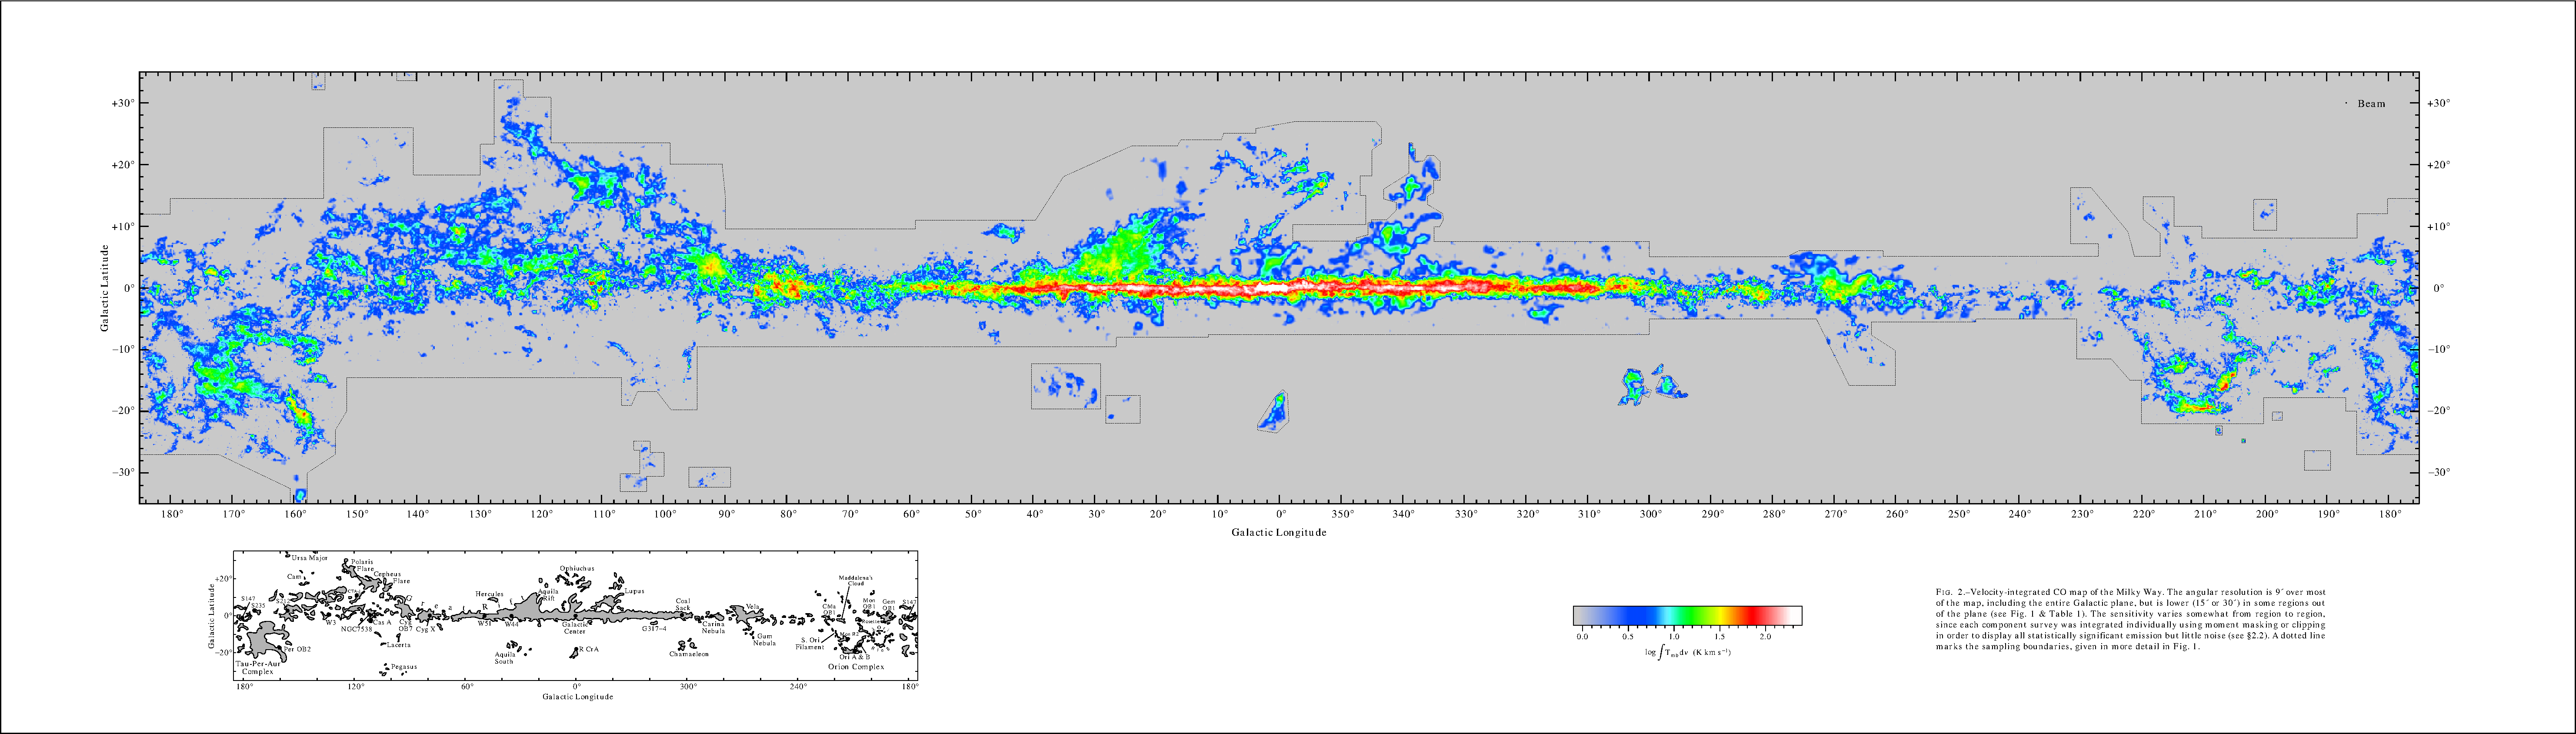
\includegraphics[width=17cm]{images/CO_long_lat.pdf}
	\caption{Ολοκληρωμένη ως προς τις ταχύτητες εκπομπή του \ce{CO} ως προς τις γαλαξιακές συντεταγμένες (Dame, Hartmann, \& Thaddeus (2001))}
	
		\centering
		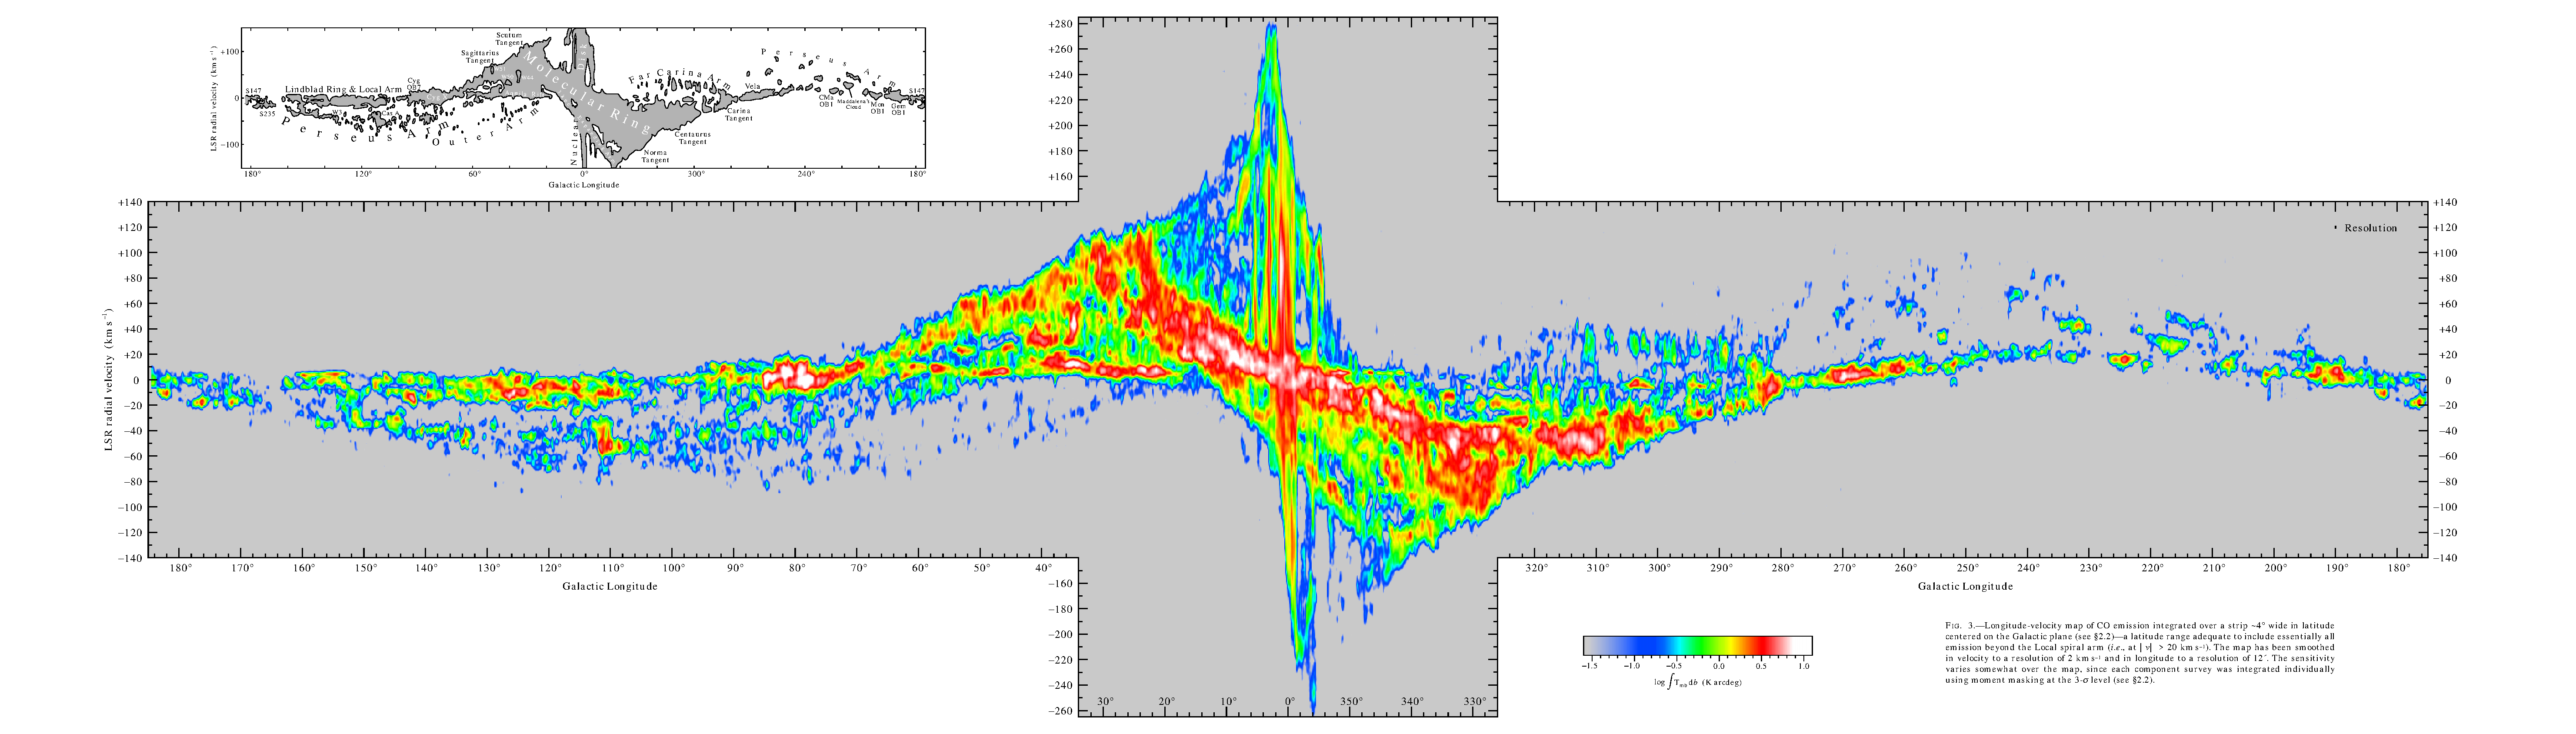
\includegraphics[width=17cm]{images/CO_long_vel.pdf}
		\caption{Εκπομπή του \ce{CO} ως προς το γαλαξιακό μήκος (Dame, Hartmann, \& Thaddeus (2001))}
\end{figure}

Εφόσον το \ce{H2} είναι δύσκολο να το παρατηρήσουμε χρησιμοποιούμε το Μονοξείδιο του Άνθρακα \ce{CO} για να χαρτογραφήσουμε το μοριακό αέριο. Το \ce{CO} είναι το δεύτερο σε αναλογία μόριο στο Σύμπαν (μετά το \ce{H2}) και έχει μόνιμη διπολική ροπή άρα έχουμε περιστροφικές ενεργειακές μεταβάσεις με $\Delta J=\pm 1$ πράγμα του επιτρέπει να εκπέμπει σημαντικά στο ραδιοφωνικό φάσμα. 
Σε αντιστοιχία με τη διαδικασία που κάναμε στη παράγραφο~(\ref{par:H2}) βρίσκουμε για το \ce{CO} για τη χαμηλότερη μετάβαση $J=1\rightarrow 0$ $\Delta E=4.8\times 10^{-4} eV$ η οποία αντιστοιχεί σε θερμοκρασία $5.5 \, K$. Η μετάβαση αυτή αποδίδει ένα ραδιοφωνικό φωτόνιο στα $2.6 \, mm$ και ο συντελεστής Einstein για την αυθόρμητη αποδιέγερση είναι $A_{10}=7.5\times 10^{-8} \, s^{-1}$.

Ο κύριος μηχανισμός διέγερσης ενός μορίου \ce{CO} στη $J=1$ είναι μέσω της σύγκρουσης του με ένα μόριο \ce{H2}. Αφού διεγερθεί η αποδιέγερση του μπορεί να γίνει είτε εκπέμποντας ένα φωτόνιο στα $2.6 \, mm$ σε περιοχές με χαμηλή συνολική πυκνότητα είτε μεταφέροντας την ενέργεια του σε ξανά σε ένα μόριο \ce{H2} χωρίς να εκπεμφθεί φωτόνιο σε περιοχές με μεγάλη συνολική πυκνότητα. Για να βρούμε την κρίσιμη πυκνότητα όπου διαχωρίζονται αυτές οι δύο περιοχές θεωρούμε ότι η πιθανότητα αυθόρμητης εκπομπής $A_{ij}$ της μετάβασης $i\rightarrow j$ είναι ίση με τη πιθανότητα εκπομπής λόγω σύγκρουσης $n \, \gamma _{ij}$. Επομένως η κρίσιμη πυκνότητα βρίσκεται:
\begin{equation}
n_{crit}=\frac{A_{ij}}{\gamma _{ij}}
\end{equation} 

Για μια τυπική θερμοκρασία $T=10 \, K$ βρίσκουμε $n_{crit}=2\times 10^3 \,cm^{-3}$.

\begin{table}
	\caption{Τα πιο συνήθη μόρια και οι πιο χρήσιμες γραμμές εκπομπής τους}
	\begin{tabular}{p{1.2cm} p{1.6cm} p{2.8cm} p{1.4cm} p{1.cm} p{2.cm} p{2.cm}}
		\toprule
		\multirow{2}{*}{Μόριο}& \multirow{2}{*}{Αναλογία}  & \multirow{2}{*}{Μετάβαση} & \multirow{2}{*}{$\lambda$} & $T$ & $A_{ij}$ & $n_{crit}$ \\ 
		 & & & & $(K)$ & $(s^{-1})$ & $ (cm^{-3}) $ \\
		\midrule
		\ce{H2} & $1$ & $1\to 0 \ S(1)$ & $2.1 \ \mu m$ & $6600$ & $8.5\e{-7}$ & $7.8\e{7}$ \\
		\ce{CO} & $8\e{-5}$ & $J=1\to 0$ & $2.6 \ mm$ & $5.5$ & $7.5\e{-8}$ & $3.0\e{3}$ \\
		\ce{OH} & $3\e{-7}$ & $^{2} \Pi _{3/2};J=3/2$ & $18 \ cm$ & $0.08$ & $7.2\e{-11}$ & $1.4\e{0}$\\
		\ce{NH3} & $2\e{-8}$ & $(J,K)=(1,1)$ & $1.3 \ cm$ & $1.1$ & $1.7\e{-7}$ & $1.9\e{4}$ \\
		\ce{H2CO} & $2\e{-8}$ & $2_{12}\to 1_{11}$ & $2.1 \ mm$ & $6.9$ & $5.3\e{-5}$ & $1.3\e{6}$ \\
		\ce{CS} & $1\e{-8}$ & $J=2\to 1$ & $3.1\ mm$ & $4.6$ & $1.7\e{-5}$ & $4.2\e{5}$ \\
		\ce{H2O} &  & $6_{16}\to 5_{23}$ & $1.3 \ cm$ & $1.1$ & $1.9\e{-9}$ & $1.4\e{3}$ \\  
		\bottomrule		
	\end{tabular}
\end{table}

\chapter{Γέννηση αστέρων στα μοριακά νέφη}
Σε αυτό το κεφάλαιο θα παρουσιάσουμε τις κυριότερες θεωρίες δημιουργίας πρωτοαστέρων μέσα στους πυρήνες των μοριακών νεφών και την επίδραση τους στο περιβάλλον του μοριακού νέφους.

\section{Κατάρρευση του μοριακού Πυρήνα}
Η δημιουργία των νέων αστέρων, σύμφωνα με όλες τις ενδείξεις, τροφοδοτείται από τη βαρυτική κατάρρευση των πυκνότερων περιοχών των μοριακών νεφών, των μοριακών πυρήνων. Παρακάτω θα αναφερθούμε, χωρίς να επεκταθούμε, στις κυρίαρχες διαδικασίες κατάρρευσης αυτών των πυρήνων.

\subsection{Αρχικές συνθήκες}
Σαν αρχικές συνθήκες της κατάρρευσης του πυκνού μοριακού πυρήνα θα χρησιμοποιήσουμε τα τυπικά φυσικά χαρακτηριστικά όπως έχουν ανιχνευθεί από παρατηρήσεις αλλά και κάποιες θεωρητικές προσεγγίσεις με βάση αυτά.

\textbf{Φυσικά Χαρακτηριστικά πυκνών μοριακών Πυρήνων:}

\begin{tabular}{|c l}
	Μάζα: & $1$ \sm \\
	Ακτίνα: & $0.1 \ pc$ \\
	Θερμοκρασία: & $10 \ K$ \\
	Πυκνότητα: & $10^{-19} \ g \, cm^{-3}$ \\
	Ποσοστό Ιονισμού: & $10^{-7}$ 
\end{tabular}

\subsubsection{Σφαίρα Bonnor-Ebert}
Η σφαίρα Bonnor-Ebert είναι η θεωρητική κατασκευή μιας ισόθερμης σφαίρας όπου η βαρύτητα εξισορροπείται από την εσωτερική πίεση. Δηλαδή ισχύουν οι εξισώσεις:
\begin{align}
\frac{Gm}{r^2} &+\frac{1}{\rho}\frac{dP}{dr}=0 \text{ Εξίσωση Κίνησης}\\
\frac{dm}{dr} &= 4 \pi r^2 \rho \text{ Εξίσωση διατήρησης της Μάζας}\\
P &= c_s ^2 \rho \text{ Καταστατική Εξίσωση}
\end{align}

Συνδυάζοντας και τις τρείς έχουμε:
\begin{equation}
\frac{1}{r^2}\frac{d}{dr} \left( r^2 c_s ^2 \frac{d \ln \rho}{dr}\right)  = -4 \pi G \rho
\end{equation}

Η λύση της οποίας μας δίνει τη πυκνότητα συναρτήση της ακτίνας μέσα στο μοριακό πυρήνα:
\begin{equation}
\label{eq:B-E_density}
\rho (r) =\frac{c_s ^2}{2 \pi G} \frac{1}{r^2}
\end{equation}

\subsection{Μαγνητικά πεδία και ύλη}
\label{par:frozenmagneticfield}
Όπως έχουμε αναφέρει προηγουμένως τα μαγνητικά πεδία φαίνεται να παίζουν σημαντικό ρόλο στη διαδικασία της βαρυτικής κατάρρευσης αλλά κυρίως στην αλληλεπίδραση του πρωτοαστέρα με το άμεσο περιβάλλον του.

Η προσέγγιση που έχουμε για την αλληλεπίδραση της ιονισμένης ύλης με τα μαγνητικά πεδία, είναι αυτή της μαγνητοϋδροδυναμικής, δηλαδή τη σύνδεση των υδροδυναμικών εξισώσεων διατήρησης (μάζα, ορμή, ενέργεια), με τις εξισώσεις του Maxwell.  

Η πολυπλοκότητα των εξισώσεων αυτών επιτρέπει την ακριβή λύση μόνο ειδικών υπεραπλουστευμένων περιπτώσεων, γι αυτό και χρησιμοποιούνται κυρίως αριθμητικοί κώδικες για την επίλυση τους.

Όμως εκτός από τη πολυπλοκότητα, ένα άλλο σοβαρό πρόβλημα που αντιμετωπίζουμε είναι η δυσκολία στο να μετρήσουμε και να χαρτογραφήσουμε το μαγνητικό πεδίο στα μοριακά νέφη και ειδικότερα στους πυκνούς πυρήνες που θα μελετήσουμε σε αυτό το κεφάλαιο. Ένα εύρος τιμών του μαγνητικού πεδίου στα μοριακά νέφη είναι $5-10\ \mu G$ για πυκνότητες κάτω των $10^3 \ cm^{-3}$. Για πυκνότητες άνω των $10^3 \ cm^{-3}$ (όπως για παράδειγμα στους πυρήνες) το μαγνητικό πεδίο δίνεται από την σχέση $B\propto \sqrt{n}$ \cite{crucher_2007}.

\subsubsection{Εξίσωση Επαγωγής}
Το μαγνητικό πεδίο προσφέρει στα μοριακά νέφη ακόμα μια δύναμη υποστήριξης, μαζί με την θερμική πίεση και τη περιστροφή, απέναντι στη βαρύτητα. Η φυσική βάση που επιτρέπει στα μαγνητικά πεδία να πέρνουν ενεργό μέρος σε αυτή τη διαδικασία είναι το φαινόμενο του "παγώματος" του μαγνητικού πεδίου μέσα στην ύλη.

Το φαινόμενο αυτό "συνδέει" την ύλη με το μαγνητικό πεδίο, έτσι καθώς η πρώτη συμπιέζεται λόγω βαρύτητας συμπιέζει μαζί της και τις δυναμικές γραμμές του πεδίου με αποτέλεσμα αυτό τοπικά να αυξάνεται.

Για να δούμε πως χτίζεται το φαινόμενο του "παγωμένου" μαγνητικού πεδίου πρέπει να κοιτάξουμε την εξίσωση επαγωγής:
\begin{equation}
\pt{\bb} = \nn \times (\vv \times \bb) -\nn \times \left( \frac{c^2}{4 \pi \sigma} \nn \times \bb \right) 
\end{equation}
όπου  $\bb$ το μαγνητικό πεδίο και $\sigma$ η είδική ηλεκτρική αγωγιμότητα.
Η εξίσωση της επαγωγής μας δίνει τη χρονική μεταβολή του πεδίου συναρτήσει ενός όρου μεταφοράς (δηλαδή τη μεταβολή της ροής του ιονισμένου υλικού) και ενός όρου διάχυσης (ωμική διάχυση).

Για ένα μοριακό νέφος παρά το χαμηλό ποσοστό ιονισμένης ύλης (σε σχέση με την ουδέτερη) αποδεικνύεται ότι ο όρος διάχυσης είναι αμελητέος, \footnote{Λόγω των κρούσεων του ιονισμένου και του ουδέτερου υλικού, εμφανίζεται ένας άλλος όρος διάχυσης, η διπολική διάχυση, για την οποία θα μιλήσουμε στη συνέχεια.} άρα η χρονική εξέλιξη του μαγνητικού πεδίου καθορίζεται από τη κίνηση του ιονισμένου ρευστού καθιστώντας το "παγωμένο".


\subsection{Ισόθερμη κατάρρευση}
Μόλις ο πυρήνας γίνει βαρυτικά ασταθής και ξεκινάει να καταρρέει, το ενεργειακό πλεόνασμα (που κερδίζεται από τη βαρυτική δυναμική ενέργεια) μετατρέπεται σε θερμότητα.
Η θερμότητα αυτή μεταφέρεται από τα μόρια στους κόκκους σκόνης που την απελευθερώνουν μέσω ακτινοβολίας στο Υπέρυθρο με αποτέλεσμα η θερμοκρασία του καταρρέοντος υλικού να παραμένει σταθερή. Αυτή η φάση κατάρρευσης του πυρήνα ονομάζεται \textbf{ισόθερμη φάση} και χαρακτηρίζεται από την ελεύθερη πτώση του υλικού στη κεντρική περιοχή.

\subsubsection{Ελεύθερη Πτώση}
Όσο η κεντρική πυκνότητα παραμένει μικρότερη από $10^{-13} \ g \, cm^{-3}$\footnote{Δηλαδή όσο το οπτικό βάθος είναι $\tau<<1$. Το οπτικό βάθος συνδέεται με τη πυκνότητα από τη σχέση $\tau \simeq k \rho R$ όπου $k$ ο δείκτης αδιαφάνειας} το γύρω υλικό θα καταρρεύσει σε χρονική κλίμακα ελεύθερης πτώσης $t_{ff} \propto (G \rho)^{-1/2} \sim 10^5 \ yr$. 
Ο ρυθμός εισροής μάζας μπορεί να υπολογιστεί μέσω ανάλυσης κλίμακας: 
\begin{equation}
\dot{M} \sim \frac{M}{t_{ff}} \sim \frac{\rho R^3}{(G \rho)^{-1/2}} \sim \frac{\rho \frac{c_s ^3}{(G \rho)^{3/2}}}{(G \rho)^{-1/2}} \sim \frac{c_s ^3}{G} \simeq 10^-6 \  M_{\odot} \, yr^{-1} 
\end{equation}
όπου για την ακτίνα χρησιμοποιήσαμε την ακτίνα $R \sim c_s t_{ff} \sim r_{jeans}$ η οποία διαχωρίζει το προς κατάρρευση υλικό του πυρήνα, με το εξωτερικό.


Από τη σχέση (\ref{eq:B-E_density}) $\rho \sim r^{-2} \rightarrow m \sim r$ εφόσον μας ενδιαφέρει η κατανομή της πυκνότητας στο "εξωτερικό" του πρωτοαστέρα άρα: 
\begin{equation}
\dot{M} \sim \frac{m}{t_{ff}} \sim m \rho^{1/2} \sim const.
\end{equation}
Άρα ο ρυθμός εισροής μάζας είναι σταθερός\footnote{Στη πραγματικότητα ο ρυθμός εισροής δεν είναι σταθερός, γι αυτό και χρησιμοποιείτε η χρονοεξαρτώμενη παραλλαγή $\dot{M}=\frac{c_s ^3}{G} e^{t/\tau}$ όπου $\tau$ μια χρονική κλίμακα όπου ο αστέρας έχει εισέλθει στη κύρια ακολουθία} κατά τη διάρκεια της ισόθερμης κατάρρευσης.

\subsection{Αδιαβατική Κατάρρευση}
Όταν η κεντρική περιοχή ξεπεράσει σε πυκνότητα τα $10^{-13} \ g \, cm^{-3}$ τότε η κατάρρευση σταματάει να είναι ισόθερμη αφού τα εσωτερικά στρώματα του πυρήνα γίνονται οπτικά αδιαφανή μην επιτρέποντας στο πλεόνασμα της ενέργειας να αποδράσει μέσω της ακτινοβολίας. Έτσι η κεντρική θερμοκρασία και η πίεση αυξάνονται.
Στη θερμοκρασία των $1000 \ K$ οι περισσότεροι κόκκοι εξαερώνονται έτσι δεν μπορούν πια να απορροφήσουν τη θερμότητα από τα μόρια που διεγείρονται.

Η καταστατική εξίσωση είναι τώρα αδιαβατική με $\frac{d \log T}{d \log \rho} = (\gamma-1) \simeq 0.4$ για το μοριακό Υδρογόνο με 5 βαθμούς ελευθερίας. Η κεντρική πίεση σε αυτό το σημείο υπερνικάει τη βαρύτητα και η κατάρρευση επιβραδύνεται δημιουργώντας ένα πρωτοαστέρα (δηλαδή ένα κεντρικό πυρήνα με υδροστατική ισορροπία) με μάζα τάξης $10^{-2}$ \sm, θερμοκρασίας $200 \ K$ και πυκνότητας $10^{-10} \ g \, cm^{-3}$.
Η ξαφνική επιβράδυνση της κατάρρευσης δημιουργεί ένα κρουστικό κύμα σε μια ακτίνα $4 \ AU$

Η εισροή μάζας στο πρωτοαστέρα αυξάνει τη πυκνότητα στο πύρηνα του στα $10^{-8} \ g \, cm^{-3}$ σε μια θερμοκρασία $1600 \ K$, όπου το \ce{H2} διασπάται μειώνοντας τον αδιαβατικό δείκτη στη τιμή $\gamma \simeq 1.1$ με αποτέλεσμα την επανεκκίνηση της κατάρρευσης με ταχύτητες αντίστοιχες της ελεύθερης πτώσης. Καθώς ολόκληρο το \ce{H2} διασπάται ο αδιαβατικός δείκτης συγκλίνει κοντά στη τιμή $5/3$ ενός αερίου ουδέτερου \ce{H} και \ce{He}. Η κεντρική θερμοκρασία σε αυτό το στάδιο έχει φτάσει στους $8000 \ K$.

Ο πρωτοαστέρας θα αποκτήσει ξανά υδροστατική ισορροπία όταν η πυκνότητα στο πυρήνα του γίνει $10^{-2} \ g \, cm^{-3}$ και η θερμοκρασία $20000 \ K$. Ο πρωτοαστέρας εξακολουθει να έχει σε αυτό το σημείο μάζα $10^{-2}$ \sm ενώ ένα νέο κρουστικό κύμα δημιουργείται σε απόσταση μερικών $R_{\odot}$. 

\subsection{Φάση Προσαύξησης}
Αν και ο πρωτοαστέρας βρίσκεται πια σε φάση Υδροστατικής ισορροπίας η πλειοψηφία της αρχικής μάζας του μοριακού πυρήνα συνεχίζει να προσαυξάνεται σε αυτόν προσκρούοντας πάνω στο κρουστικό κύμα που περιγράψαμε παραπάνω. 
Η κινητική ενέργεια της ύλης που φτάνει σε αυτό το σημείο μετατρέπεται σχεδόν εξ ολοκλήρου σε ακτινοβολία, δηλαδή $\frac{u^2}{2}=\frac{GM}{R}$, άρα αν πολλαπλασιάσουμε με $\dot{M}$ βρίσκουμε την εισροή ενέργειας ανά δευτερόλεπτο. Αν υποθέσουμε επιπλέον ότι ολόκληρη αυτή η ενέργεια μετατρέπεται σε ακτινοβολία από το κρουστικό κύμα: 
\begin{equation}
L_{acc} \simeq \frac{GM\dot{M}}{R}
\end{equation}

Ταυτόχρονα και ο ίδιος ο πρωτοαστέρας ακτινοβολεί με ρυθμό:
\begin{equation}
L_{star}=4 \pi R^2 \sigma T_{eff} ^4
\end{equation}
σύμφωνα με το νόμο Stefan-Boltzmann.

Για πρωτοαστέρες μικρής και μέσης μάζας η λαμπρότητα λόγω πρόσπτωσης $L_{acc}$ κυριαρχεί έναντι της λαμπρότητας του ίδιου του πρωτοαστέρα.


\section{Κατάρρευση περιστρεφόμενου και μαγνητισμένου μοριακού πυρήνα}
Παραπάνω όπου θεωρήσαμε ένα αρχικό σφαιρικό, μη-περιστρεφόμενο, μη-μαγνητισμένο πυρήνα, ασχολούμασταν με την "διαμάχη" της βαρύτητας με τη θερμική πίεση του αερίου. 

Στη περίπτωση όπου το νέφος έχει μια αρχική γωνιακή ταχύτητα, βρίσκεται μέσα σε μαγνητικό πεδίο και έχει μάζα μεγαλύτερη από τη κρίσιμη (βλέπε και παράγραφο~\ref{par:VirialMass}) θα καταρρεύσει σε γενικές γραμμές όπως αναλύσαμε στη κλασική περίπτωση.

Η μεγαλύτερη διαφορά με την κλασική προσέγγιση εμφανίζεται κυρίως στη φάση της πρόσπτωσης της ύλης στο πρωτοαστέρα όπου η περιστροφή και το μαγνητικό πεδίο παίζει σημαντικό ρόλο.

\subsection{Η περίπτωση αργά περιστρεφόμενου πυρήνα}
Θεωρούμε ότι το νέφος είναι αρχικά σφαιρικά συμμετρικό με μικρή γωνιακή ταχύτητα και ότι η κατάρρευση έχει δημιουργήσει ήδη τον κεντρικό πρωτοαστέρα.
Το υλικό εκτελεί ελεύθερη πτώση ξεκινώντας από τη θέση $(r_0,\theta _0)$, όπου $\theta _0$ η γωνία από τον άξονα περιστροφής, προς το κεντρικό πυρήνα διατηρώντας την ειδική στροφορμή του $j=\Omega r_0 ^2 \sin \theta_0$, και με σταθερή επιτάχυνση $\dot{M} \simeq \frac{c_s ^3}{G}$.   

\begin{figure}[h]
	\centering
	\includegraphics[width=\medpage]{images/disk2.ps}
	\caption{Ο μηχανισμός δημιουργίας του δίσκου προσαύξησης ενός περιστρεφόμενου καταρρέοντος νέφους}
\end{figure}


Αν δεχθούμε ότι η κατάρρευση είναι αξισυμμετρική ως προς τις γωνίες $\phi$ και ως προς τη ισημερινή επιφάνεια $\theta = \pi/2$ είναι προφανές ότι το υλικό "από πάνω" θα συγκρουστεί με το "από κάτω" πάνω στο στο ισημερινό επίπεδο, και μάλιστα αποδεικνύεται ότι για κάθε αρχικό σημείο $(r_0,\theta _0)$ το σημείο της σύγκρουσης αντιστοιχεί σε ένα σημείο $(r_{ct},\pi/2)$, όπου:
\begin{equation}
r_{ct}=\frac{j^2}{GM}=\frac{\Omega^2 r_0 ^4 \sin ^2 \theta_0}{GM}
\end{equation}
Το αποτέλεσμα θα είναι η δημιουργία μια κατανομής πυκνότητας:
\begin{equation}
\rho (r,\theta) =\frac{\dot{M}}{4 \pi \sqrt{G M r^3}}\left(1+\frac{\cos \theta}{\cos \theta _0}\right)^{-1/2} \left( \frac{\cos \theta}{\cos \theta _0} + \frac{2 R_c \cos^2 \theta _0}{r} \right) ^{-1} 
\end{equation}

Μέσω αυτής της διαδικασίας έχουμε τη δημιουργία ενός δίσκου προσαύξησης όπου η ύλη ακολουθεί κεπλεριανές τροχιές γύρω από τον αστέρα.

Άρα βλέπουμε ότι τα σωματίδια με μικρές αρχικές γωνίες $\theta _0 \to 0$, δηλαδή με μικρή στροφορμή, θα συγκρουστούν πάνω στην επιφάνεια του πρωτοαστέρα, ενώ τα σωματίδια που βρίσκονται από την αρχή στο ισημερινό επίπεδο θα είναι αυτά που θα δημιουργήσουν τις τελευταίες τροχίες του. 

Έτσι μπορούμε να υπολογίσουμε την ακτίνα ολόκληρου του δίσκου:
\begin{equation}
R_c=\frac{\Omega^2 r_0 ^4}{GM} = m_0 \frac{\Omega^2 (c_s t)^4}{G \dot{M} t} =m_0 \Omega ^2 c_s t^3
\end{equation}
όπου $m_0$ μια σταθερά, η οποία βρίσκεται από την αναλυτική λύση $m_0=0.058$. 

Για τυπικές τιμές ενός πρωτοαστέρα, ($M=1$, $M_{\odot}$, $\dot{M}=10^{-5} \ M_{\odot} \, yr^{-1}$, $c_s =0.35\ km\, s^{-1}$, $r_0 = 1.5 \e{15}\ cm$) βρίσκουμε ότι $R_c \simeq 44\ A.U.$.  

\subsection{Περίπτωση κατάρρευσης μαγνητισμένου νέφους}
Στη παράγραφο \ref{par:frozenmagneticfield} αναφέραμε τη "κοινή" συμπεριφορά μαγνητικού πεδίου και ιονισμένης ύλης. Στη συνέχεια θα αναφερθούμε περιγραφικά στο πως αυτή η συμπεριφορά επιδρά στη βαρυτική κατάρρευση του πυκνού μοριακού πυρήνα.

Το υπό κατάρρευση μοριακό νέφος αποτελείται σε πολύ μικρό ποσοστό από ιονισμένη ύλη. Άρα δεν μπορούμε να επικαλεστούμε την προσέγγιση του παγωμένου μαγνητικού πεδίου. 

Εν προκειμένου έχουμε δύο διαφορετικές κινήσεις μέσα στο νέφος: το ιονισμένο αέριο κινείται κατά μήκος των μαγνητικών γραμμών, ενώ το ουδέτερο κινείται λόγω της βαρύτητας και της θερμικής πίεσης ανεξάρτητα του μαγνητικού πεδίου.
Όμως οι δύο αυτοί πληθυσμοί σωματιδίων εφόσον αλληλεπιδρούν μεταξύ τους μέσω συγκρούσεων επηρεάζουν εν τέλει και τις δύο αυτές κινήσεις. Το φαινόμενο αυτό ονομάζεται \textbf{διπολική διάχυση}.

Έστω ότι ο πυκνός μοριακός πυρήνας βρίσκεται εντός ενός ομογενούς αρχικού μαγνητικού πεδίου $B_0$. Καθώς ξεκινάει η κατάρρευση τα ιονισμένα και τα ουδέτερα σωματίδια είναι ελεύθερα να κινηθούν κατά μήκος των μαγνητικών δυναμικών γραμμών. 

Παρόλαυτα στη διεύθυνση κάθετα στο μαγνητικό πεδίο τα ουδέτερα σωματίδια συγκρούονται με τα ιονισμένα, με αποτέλεσμα η κατάρρευση σε αυτή τη διεύθυνση να επιβραδύνεται και τα ιόντα να παρασύρονται από τα ουδέτερα. Όμως καθώς το μαγνητικό πεδίο είναι παγωμένο μέσα στην ιονισμένη ύλη, οι δυναμικές του γραμμές συγκλίνουν και αυτές προς το κέντρο κατάρρευσης, αυξάνοντας τοπικά το μαγνητικό πεδίο, ενώ η ίδια η καμπύλωση τους ασκεί δύναμη αντίθετη στη κατάρρευση λόγω της μαγνητικής τάσης. 

Εν τέλει, όπως και με τη περίπτωση του περιστρεφόμενου πυρήνα, το μαγνητικό πεδίο δημιουργεί ένα δίσκο γύρω από το πρωτοαστέρα, που όμως δεν έχει της δυναμικές ιδιότητες του δίσκου προσαύξησης.


\begin{figure}[h]
	\centering
	\includegraphics[height=7.5cm]{images/magnetic_collapse.ps}
	\caption{Ο μηχανισμός κατάρρευσης ενός μαγνητισμένου νέφους και η δύναμη λόγω καμπυλότητας των μαγνητικών γραμμών}
\end{figure}


\section{Δίσκοι Προσαύξησης}
Αναφερθήκαμε προηγουμένως στο πως ένα αρχικά περιστρεφόμενο μοριακό νέφος θα δημιουργήσει κατά τη κατάρρευση του ένα δίσκο προσαύξησης γύρω από τον πρωτοαστέρα. Σε αυτή τη φάση ο πρωτοαστέρας έχει μάζα μόλις $10^{-2}$ \sm, κάτι το οποίο σημαίνει ότι μάζα προσπίπτει στον αστέρα μέσω του δίσκου.

Αν θεωρήσουμε ότι ένας στοιχειώδης δακτύλιος πάχους $\delta r$ του δίσκου σε απόσταση $r$ από πρωτοαστέρα μάζας $M$ κινείται με κεπλεριανή ταχύτητα $v_{\phi}=\sqrt{\frac{GM}{r}}$ τότε η ειδική στροφορμή του θα είναι $r \, v_{\phi}=\sqrt{GMr}$ δηλαδή θα αυξάνεται με την απόσταση. Άρα για να καταφέρει ο δακτύλιος αυτός να φτάσει το πρωτοαστέρα θα πρέπει η στροφορμή του συνεχώς να ελαττώνεται, δηλαδή να υπάρχει κάποιος μηχανισμός ο οποίος μέσω κάποιας ροπής δύναμης θα οδηγεί σε απώλεια στροφορμής.

Οι πιο πιθανοί τέτοιοι μηχανισμοί είναι: η εσωτερική τριβή του ρευστού του δίσκου, η επίδραση του ενεργού ιξώδες λόγω τυρβώδους ροής και η απώλεια στροφορμής μέσω μαγνητισμένων εκροών.


\section{Η επίδραση των πρωτοαστέρων στο περιβάλλον τους}

Από τις πρώτες στιγμές της δημιουργίας τους οι αστέρες επηρεάζουν σημαντικά το περιβάλλον τους μέσω δυναμικών μηχανισμών όπως οι εκροές μάζας (Outflows, Jets) και ο αστρικός άνεμος αλλά και λόγω της επίδρασης της ακτινοβολίας (ιονισμός Υδρογόνου). Η επίδραση αυτών των μηχανισμών στο περιβάλλον τους έχει πολύ μεγάλη εξάρτηση από τη μάζα των πρωτοαστέρων, καθώς οι αστέρες μεγάλης μάζας έχουν πολύ ισχυρότερη επιρροή από τους μέσης ή μικρής μάζας.

Συγκεκριμένα οι μηχανισμοί εκροών μάζας εμφανίζονται σε όλους τους πρωτοαστέρες ανεξαρτήτως μάζας, τηρουμένων πάντα των αναλογιών. Οι μηχανισμοί αυτοί είναι απόρροια της διαδικασίας προσαύξησης των πρωτοαστέρων και άρα έχουν περιορισμένο χρόνο ζωής με αποτέλεσμα η επίδραση τους να γίνεται αισθητή μόνο στο σχετικά γειτονικό περιβάλλον (σε αποστάσεις μερικών pc) \cite{Yildiz_2015}. 

Απεναντίας οι αστρικοί άνεμοι, και τα φωτόνια υψηλών ενεργειών που δημιουργούνται μόνο στους αστέρες μεγάλης μάζας, επιδρούν στο περιβάλλον για πολύ μεγαλύτερο χρονικό διάστημα με καταστροφικές συνέπειες για πολύ μεγάλο μέρος του μοριακού νέφους.


\subsection{Πίδακες και εκροές υλικού}
Οι κυρίαρχες θεωρίες για την δημιουργία των πιδάκων υλικού (jets) βασίζονται στο συνδυασμό της περιστροφικής κίνησης του δίσκου και του αστέρα και στο διπολικό μαγνητικό πεδίο του αστέρα. 
Σύμφωνα με τα υπάρχουσα μοντέλα υλικό υπό τη μορφή αστρικού ανέμου από το δίσκο ευθυγραμμίζεται και επιταχύνεται κάθετα στο δίσκο και στη διεύθυνση του άξονα περιστροφής δημιουργώντας μια σχετικά στενή δομή που διατηρείται για αρκετά μεγάλες αποστάσεις.

Οι πίδακες τροφοδοτούν με ενέργεια όχι μόνο το άμεσο περιβάλλον του πρωτοαστέρα αλλά και αέριο του μοριακού νέφους πέρα από τον αρχικό πυρήνα. Η ενέργεια αυτή δημιουργεί τύρβη στο νέφος


\subsection{Αστέρες μεγάλης μάζας}
Οι μεγάλης μάζας αστέρες είναι αστέρες των οποίων οι μάζες ξεπερνούν τις 8 \sm με φασματικούς τύπους O και B, χαρακτηρίζονται από ταχύτατους ρυθμούς εξέλιξης \footnote{Οι μεγάλης μάζας αστέρες ξεκινούν τη καύση του Υδρογόνου ενώ βρίσκονται ακόμα στη φάση της προσαύξησης, ενώ και ο χρόνος ζωής τους δεν ξεπερνάει τα $3 \times 10 ^7 yr$} με τεράστιες λαμπρότητες ($L_* > 10^4 L _ \odot$) και επιφανειακή θερμοκρασία $>10 ^5 \ K$.

\subsubsection{Περιοχές HII}
\label{par:HII regions}
Λόγω των πολύ υψηλών θερμοκρασιών, οι OB αστέρες εκπέμπουν υψηλό αριθμό φωτονίων υψηλών ενεργειών (μεγαλύτερες από το όριο Lyman, στο υπεριώδες) τα οποία διασπούν το μοριακό υδρογόνο σε δύο ατομικά τα οποία τελικά θα ιονιστούν. Οι περιοχές όπου το αέριο υδρογόνο είναι ιονισμένο ονομάζονται περιοχές HII. Στις περιοχές $HII$ το πλάσμα υδρογόνου επιχειρεί συνεχώς να επανασυνδεθεί για να σχηματίσει ουδέτερα άτομα υδρογόνου αλλά εμποδίζεται από τη συνεχιζόμενη παραγωγή υπεριωδών φωτονίων.

Μπορούμε να ορίσουμε μια περιοχή μέσα στην οποία ένας αστέρας OB μπορεί να τη διατηρήσει ιονισμένη συγκρίνοντάς τη λαμπρότητά του στο υπεριώδες με το ρυθμό επανασύνδεσης των ατόμων Υδρογόνου. Μια τέτοια περιοχή ονομάζεται σφαίρα Stromgren και για μια τυπική θερμοκρασία $10^4 \ K$ και ρυθμό επανασύνδεσης $2 \e{-19} \ m^3 \,s^{-1}$ βρίσκουμε:
\begin{equation}
R_s \simeq 1.7 \, pc \left( \frac{\dot{N}_H}{10^{50} \, s^{-1}} \right)^{1/3} \left( \frac{n_0}{10^9 \, m^{-3}} \right) ^{-2/3}
\end{equation}
όπου $\dot{N}_H$ είναι ο αριθμός των φωτονίων πέρα από το όριο Lyman στη μονάδα του χρόνου και $n_0$ η αριθμητική πυκνότητα των ατόμων υδρογόνου (ανεξαρτήτως κατάστασης).

Στη πραγματικότητα καθώς το σύνορο της περιοχή HII εκκινώντας από τον πρωτοαστέρα με υπερηχητική ταχύτητα, όπως θα δείξουμε παρακάτω, θα ξεπεράσει τελικά την ακτίνα Stromgren λόγω της υψηλότερης θερμοκρασίας (άρα και πίεσης) από το κρύο περιβάλλον του ουδέτερου υδρογόνου. 

Ο χρόνος\footnote{Aν δεχθούμε ότι ο μέσος χρόνος επανασύνδεσης είναι μικρότερος από το χρόνο εξάπλωσης, το οποίο για τις πυκνότητες των περιοχών HII είναι σωστή προσέγγιση} που χρειάζεται για να δημιουργηθεί μια περιοχή HII είναι:
\begin{equation}
t_{expand} \simeq \frac{R_s}{c_{s \, HII}} \simeq 1.7\e{5} \ yr \ \f{\dot{N}_H}{10^{50} \, s^{-1}}{1/3} \f{n_0}{10^9 \, m^{-3}}{-2/3}
\end{equation}
αφού η ταχύτητα του ήχου για τις συνθήκες αυτές, δηλαδή η ταχύτητα εξάπλωσης της περιοχής HII, είναι:
\begin{equation}
c_{s \, HII} = \f{kT_{HII}}{m_{HII}}{-1/2} \simeq 12 \ km\,s^{-1}
\end{equation}

Η ταχύτητα του ήχου για το ουδέτερο αέριο υδρογόνο είναι $c_{s \, HI}\simeq 0.3 \ km \, s^{-1}$, άρα η περιοχή HII δημιουργώντας ένα κρουστικό κύμα καθώς εξαπλώνεται μέσα στο ουδέτερο υδρογόνο. 

Η διαδικασία αυτή είναι πάρα πολύ σημαντική για τη δημιουργία αστέρων. Οι δύο επικρατέστερες θεωρίες για το πώς επιδρούν οι περιοχές αυτές στη διαδικασία δημιουργίας αστέρων είναι οι ακόλουθες:
\begin{itemize}
	\item Στο μοντέλο \textbf{Collect and Collapse} \cite{whitworth_1994} καθώς το κρουστικό κύμα διασχίζει το μεσοαστρικό χώρο συγκεντρώνει και συμπιέζει την υπάρχουσα ύλη δημιουργώντας καινούργιες πυκνές δομές κάποιες από τις οποίες είναι βαρυτικά ασταθείς. Οπότε δημιουργούνται νέοι αστέρες. Οι περιοχές αυτές μπορούν να υποστηρίξουν τη δημιουργία αστέρων μεγάλης μάζας που με τη σειρά τους θα δημιουργήσουν τις δικές τους περιοχές HII και ούτω κάθε εξής.
	\item Στο μοντέλο \textbf{Radiation Driven Implosion (RDI)} \cite{bertoldi_1981} το κρουστικό κύμα συγκρούεται με προϋπάρχουσες πυκνές δομές οι οποίες εξαιτίας της αυξημένης αυτής εξωτερικής πίεσης καθίστανται βαρυτικά ασταθείς και τελικά καταρρέουν.
\end{itemize}
Η διαφορά των δύο μοντέλων έγκειται ότι στο πρώτο δημιουργούμε καινούργιες δομές ενώ στο δεύτερο οι δομές προϋπάρχουν. Θεωρείται ότι το μοντέλο Collect and Collapse κυριαρχεί σε δομές μεγάλης κλίμακας σε αντίθεση με το RDI.

\begin{figure}[h]
	\centering
	\includegraphics[height=14cm]{images/induced.ps}
	\caption{Η διαδικασία της δημιουργίας λόγω του κρουστικού κύματος πίεσης των περιοχών HII αστέρων μεγάλης μάζας OB}
\end{figure}


\chapter{Το γιγαντιαίο μοριακό νέφος W3}

\begin{figure}[h]
	\centering
	\includegraphics[width=\medpage]{images/DSS_colored.png}
	\caption{Η περιοχή του W3 και W4 στο οπτικό. DSS2 optical HEALPix survey (R=0.6μm,G=average,B=0.4μm)}
\end{figure}

Το γιγαντιαίο μοριακό νέφος W3 είναι μέρος ενός συμπλέγματος μοριακών νεφών (W3-W4-W5) στον αστερισμό της Κασσιόπης, σε απόσταση $2 \ kpc$\cite{Xu_2006},\cite{Hachisuka_2006} από τον ήλιο, στη σπείρα του Περσέα του Γαλαξία μας.

Η μάζα του εκτιμάται στις $4\e{5} \ M_{\odot}$ κάνοντας το ένα από τα πιο μαζικά μοριακά νέφη στον εξωτερικό Γαλαξία.\cite{moore_2007},\cite{polychroni_gas_2012}

Το 40\% της μάζας του νέφους είναι συγκεντρωμένη σε μιά περιοχή υψηλής πυκνότητας υπό την ονομασία High Density Layer (HDL) στην οποία βρίσκονται και οι τρείς περιοχές με την μεγαλύτερη δραστηριότητα - όσον αφορά την δημιουργία αστέρων - του W3, οι W3 Main, W3 (OH) και AFGL333. Η δομή πιθανολογείται ότι είναι αποτέλεσμα του κρουστικού κύματος μιας διευρυμένης περιοχής HII (W4 superbubble) που βρίσκεται στα ανατολικά του W3 μέσω του μηχανισμού Collect and Collapse που περιγράψαμε στη παράγραφο (\ref{par:HII regions}). Η περιοχή αυτή τροφοδοτείτε από αστρικούς ανέμους ενός σμήνους OB αστέρων (IC 1805 OB association) που βρίσκονται στη καρδιά του μοριακού νέφους W4.

Πιθανόν αποτέλεσμα της W4 HII είναι η δημιουργία του νεαρού αστρικού σμήνους IC 1795 (με ηλικία $3-5 \ Myr$)\cite{rivera-ingraham_2011}. To IC 1795 διαθέτει μερικούς αστέρες OB που έχουν δημιουργήσει ένα κέλυφος στο οποίο ανήκουν οι περιοχές W3 Main και W3 (OH).

Στη περιοχή W3 Main έχουν ανιχνευτεί πολλές πυκνές περιοχές HII που αποδίδονται σε νεαρούς αστέρες OB που δεν έχουν διαλύσει ακόμα τα κελύφη σκόνης που τους καλύπτουν. Παρότι φαίνεται ότι η W3 Main διεγέρθηκε από το IC 1795 ή τη W4 HII υπάρχουν ενδείξεις ότι μπορεί να έχει ξεκινήσει τη δημιουργία αστέρων νωρίτερα από το IC 1795\cite{feigelson_2008}. Το οποίο σημαίνει ότι μπορεί η δημιουργία αστέρων να ξεκίνησε αυθόρμητα.


\begin{figure}[h]
	\centering
	\includegraphics[width=\medpage]{images/GLIMPSE360.png}
	\caption{Η περιοχή του W3 και W4 στο υπέρυθρο, από το GLIMPSE360}
\end{figure}

Νότια από το αστρικό σμήνος IC 1795 βρίσκεται η περιοχή W3 (OH) για την οποία υπάρχουν οι ισχυρότερες ενδείξεις ότι αποτελεί προϊόν της πίεσης από το IC 1795 και τη  W4 HII. Στη περιοχή αυτή έχουμε ισχυρές εκπομπές \ce{OH} και \ce{H2O} (masers) από τις οποίες έχει μετρηθεί η απόσταση του μοριακού νέφους μέσω παράλλαξης ($1.95 \pm 0.04 \ kpc$).

Στη νότια-ανατολική γωνία του W3 και κοντινότερα στο W4 βρίσκεται η περιοχή AFGL 333 η οποία παίρνει το όνομα της από τον ομώνυμο αστέρα φασματικού τύπου B0.5 στο εσωτερικό της. 

Εκτός από τις παραπάνω περιοχές όπου πιστεύουμε ότι η διαδικασία δημιουργίας αστέρων είναι πιθανό αποτέλεσμα περιοχών HII, στη νότια-δυτική γωνία του W3 έχουμε τη πιο ισχυρή ένδειξη αυθόρμητης γέννησης αστέρων, τον αστέρα μεγάλης μάζας VES 735 με φασματικό τύπο O8.5 και ηλικία $1-2 \ Myr$ στον οποίο οφείλεται η περιοχή HII KR 140. Το χαρακτηριστικό σφαιρικό κέλυφος της KR 140 είναι διεγερμένη περιοχή όπου δημιουργούνται νέοι αστέρες. 

Βόρεια της KR 140 βρίσκεται η περιοχή KR 140-N ή Trilobite. Η μορφολογία αυτής της περιοχής είναι ενδεικτική του μοντέλου RDI \cite{rivera-ingraham_2013}. Σύμφωνα με νέες παρατηρήσεις από το Herchel Space Observatory ενδεχομένως το κρουστικό κύμα στο οποίο οφείλεται η περιοχή αυτή να προέρχεται και αυτό από το W4 HII Superbubble (Προσωπική επικοινωνία με Polychroni D.)

\begin{table}
	\caption{Παράμετροι υποπεριοχών του W3 από χαρτογράφηση του Spitzer. YSO: Υoung Stellar Object, συντομογραφία των υποψήφιων πρωτοαστέρων}
	\begin{tabular}{p{2.cm} p{2.5cm} p{1.5cm} p{2cm} p{2.2cm} p{2.5cm}}
		\toprule
		\multirow{2}{*}{Περιοχή} & Μέση απόσταση YSO & Εμβαδόν περιοχής & Μάζα Αερίου & Πυκνότητα Αερίου & Μέση Πυκνότητα YSO \\ 
		&  $(pc)$ & $(pc^2)$ & $(\e{4} \ M_{\odot})$ & $(M_{\odot} \ pc^{-2})$ & $ (pc^{-2}) $ \\
		\midrule
		All-Survey & $0.33 \pm 0.01$ & $1316$ & $6.2\pm0.005$ & $59.44\pm 0.04$ & $1.73\pm 0.001$ \\
	  W3 Main/(OH) & $0.26 \pm 0.01$ & $231.5$ & $1.4\pm0.002$ & $61.31\pm 0.08$ & $3.41\pm 0.005$ \\
	  KR 140 & $0.38 \pm 0.02$ & $853$ & $3.8\pm0.004$ & $45.38\pm 0.04$ & $1.25\pm 0.004$ \\
	  AFGL 333 & $0.34 \pm 0.02$ & $231.5$ & $1.0\pm0.002$ & $53.3\pm 0.1$ & $1.77\pm 0.004$ \\  
		\bottomrule		
	\end{tabular}
\end{table}

\begin{figure}[h]
	\centering
	\includegraphics[height=11cm]{images/aladin/crawford}
	\caption{a}
	
	\centering
	\includegraphics[height=11cm]{images/aladin/infrared-ob-co}
%	\caption{}
\end{figure}

\begin{figure}[h]
	\centering
	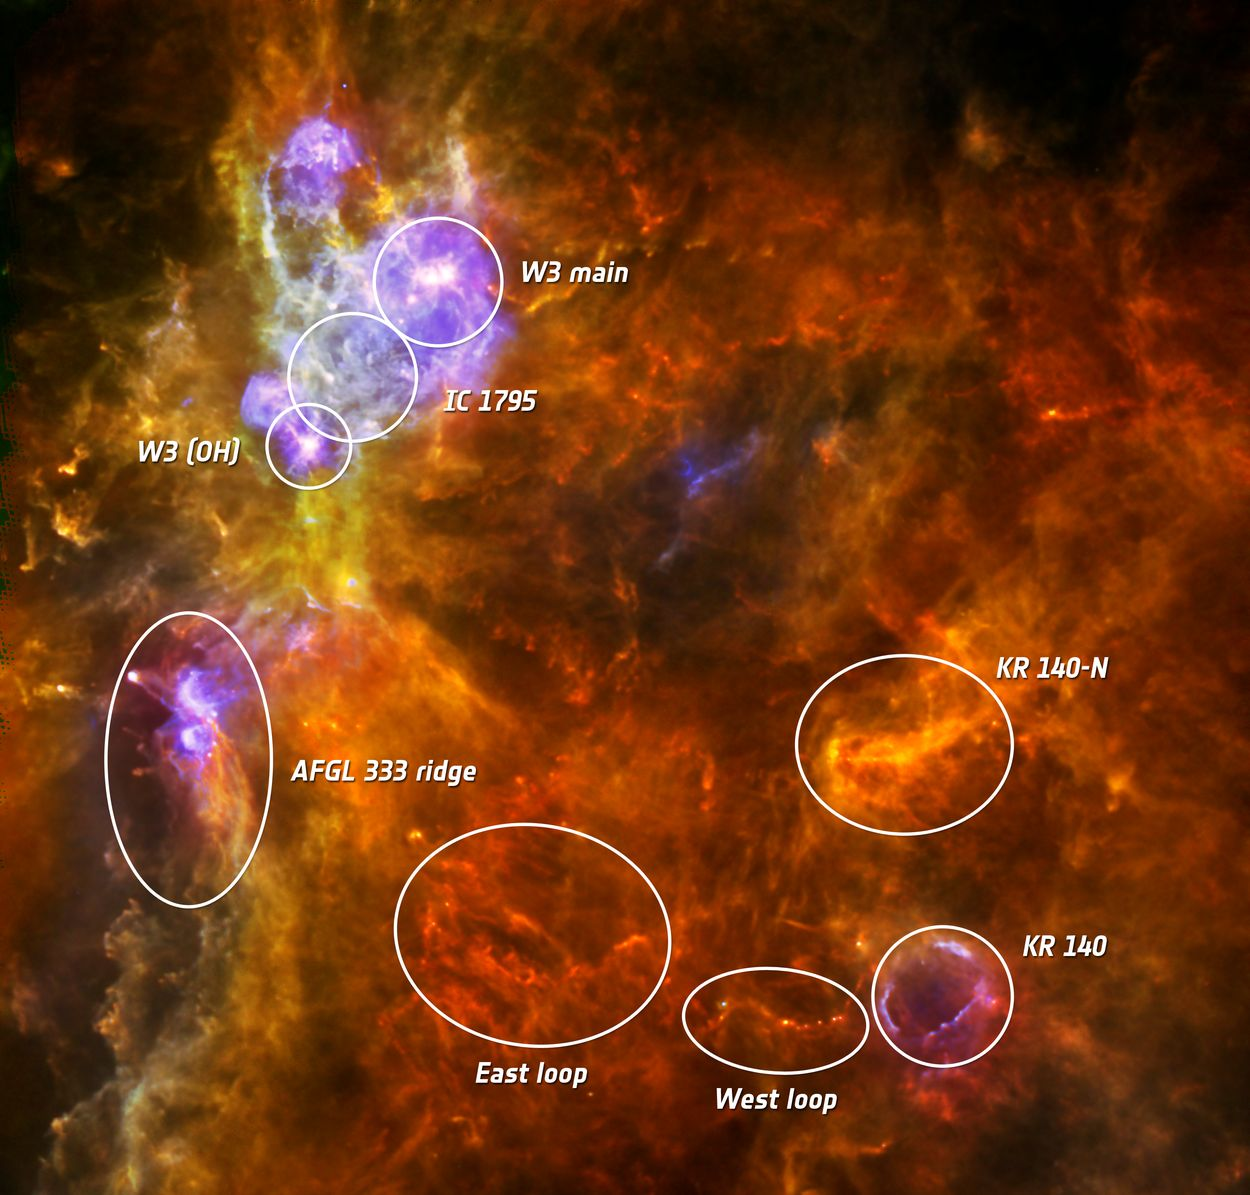
\includegraphics[width=13cm]{images/w3_70_160_250_annotated.jpg}
	\caption{Εικόνα του W3 από το Herschel (R=250 µm, B=70 µm,G=160 µm)}
\end{figure}



\chapter{Παρατηρήσεις στο ραδιοφωνικό φάσμα}

\begin{figure}[hb]
	\centering
	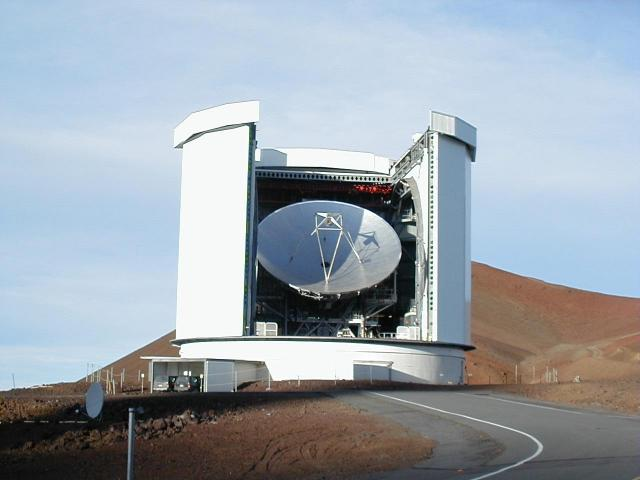
\includegraphics[width=12cm]{images/JCMT.jpg}
	\caption{Το ραδιοτηλεσκόπιο James Clerk Maxwell Telescope (JCMT)}
\end{figure}

Σκοπός τη εργασίας είναι η μελέτη των μοριακών εκροών από τους πυκνούς πυρήνες, και συγκεκριμένα στο μοριακό νέφος W3 GMC. Γι αυτό το λόγο θα χρησιμοποιήσουμε γραμμές εκπομπής του Μονοξειδίου του Άνθρακα (\ce{CO}). Το \ce{CO} είναι το δεύτερο σε αναλογία μόριο στο Σύμπαν (μετά το \ce{H2}) και λόγω της σχετικά μικρής κρίσιμης πυκνότητας χρησιμοποιείται για τη χαρτογράφησης των μεγάλης κλίμακας δομών των μοριακών νεφών, και όχι των πυρήνων. Σε αυτές τις κλίμακες οι χαμηλότερες ενεργειακά γραμμές του \ce{CO} είναι οπτικά αδιαφανείς, το οποίο σημαίνει ότι τα φωτόνια που παρατηρούμε προέρχονται από τα εξωτερικά στρώματα των νεφών.

\begin{wrapfigure}{r}{4cm}
	\begin{flushright}
		\includegraphics[height=8cm]{images/harp_photo.png}
		\caption{Το όργανο HARP (Heterodyne Array Receiver Programme)}
	\end{flushright}
\end{wrapfigure}


Συγκεκριμένα θα χρησιμοποιήσουμε τις γραμμές εκπομπής των \ce{^{12}CO} (345.796 GHz) και στα ισότοπά του \ce{^{13}CO} (330.540 GHz), \ce{C^{18}O} (329.278 GHz) -για εκπομπή από τη διεγερμένη στάθμη $J=3$ στη στάθμη $J=2$-. Οι γραμμές αυτές επιλέχθηκαν καταρχήν λόγω του ότι βρίσκονται μέσα στο παρατηρησιακό εύρος του οργάνου HARP \footnote{Το παρατηρησιακό εύρος τους HARP είναι στα 325-375 GHz. \\ Η γραμμή εκπομπής \ce{^{12}CO} $J=1\to 0$ είναι στα .} το οποίο μας προσφέρει πάρα πολύ καλή διακριτική ικανότητα $7.5\ arcsec$. 
 Οι γραμμές ισοτόπων παρατηρούνται για τον υπολογισμό του οπτικού βάθους της κύριας γραμμής καθώς και τα διαφορετικά οπτικά βάθη των ισοτόπων μας δίνουν μια εικόνα του νέφους από τα εξωτερικά στρώματα του έως τους πυρήνες εντός του.
Ο δεύτερος λόγος της επιλογής αυτών των γραμμών εκπομπής είναι ότι το CO J=3->2 είναι ευαίσθητο σε πιο θερμά υλικά, οπότε μπορούμε να παρατηρήσουμε της μοριακές εκροές οι οποίες έχουν υψηλότερες θερμοκρασίες από το γύρω περιβάλλον τους καλύτερα. (βλέπε )

Οι παρατηρήσεις αυτές έγιναν από τη Polychroni D. στο χρονικό διάστημα 2006-2008 στο ραδιοτηλεσκόπιο James Clerk Maxwell Telescope (JCMT) που βρίσκεται στη περιοχή Mauna Kea της Χαβάης σε υψόμετρο 4092 μέτρων. Όλες οι παρατηρήσεις πραγματοποιήθηκαν με καλό καιρό, με τη διαφάνεια του ουρανού στα 225 GHz $\tau _{225} <0.08$.

\bigskip

\section{Ραδιοτηλεσκόπιο JCMT}

Το κύριο κάτοπτρο του JCMT έχει διάμετρο 15 μέτρων και είναι κατασκευασμένο από 276 αυτόνομα ελαφριά πάνελ. Κάθε πάνελ αποτελείται από μια επιφάνεια λεπτού αλουμινίου που προσαρμόζεται σε τρία σημεία πάνω στον υποστηρικτικό κορμό της κεραίας ο οποίος είναι σχεδιασμένος να διατηρεί τη παραβολική του γεωμετρία απέναντι στις βαρυτικές παραμορφώσεις καθώς κινείται σε διαφορετικές γωνίες.

Για παρατηρήσεις στη μπάντα των 325-375 GHz το JCMT περιλαμβάνει δύο όργανα: το SCUBA-2 και το HARP (Heterodyne Array Receiver Programme). Για τις παρατηρήσεις μας χρησιμοποιήθηκε το  HARP μαζί με το φασματογράφο ACSIS (Auto-Correlation Spectral Imaging System). Το HARP περιλαμβάνει 16 αισθητήρες με οπτικό πεδίο $14 \ arcsec$ σε απόσταση $30 \ arcsec$. Το εύρος ζώνης του ACSIS είναι 250 Mhz άρα για τη συχνότητα 345.796 GHz του \ce{^{12}CO} $J=3\to 2$ π.χ. το εύρος αντιστοιχεί σε $250\ MHz \times 0.87\ km\,s^{-1} = 217.5\ km\,s^{-1}$\footnote{1 MHz αντιστοιχεί σε $0.87\  m\,s^{-1}$}. Δηλαδή για 8192 κανάλια έχουμε ανάλυση $26\ m\,s^{-1}$. 

\section{Παρατήρησεις και διαμόρφωση δεδομένων}
Η τεχνική παρατήρησης που χρησιμοποιήθηκε είναι η Raster Mapping η οποία είναι η καλύτερη για παρατήρηση εκτεταμένων περιοχών με σχετικά δυνατή λαμπρότητα γραμμών εκπομπής. Σε αυτή τη τεχνική το ραδιοτηλεσκόπιο σαρώνει μια ευθεία σταθερού πλάτους όσο ο δέκτης (ACSIS) βρίσκει τη μέση τιμή του εισερχόμενου σήματος ανά τακτά χρονικά διαστήματα. 


\begin{figure}[h]
	\centering
	\includegraphics[width=8cm]{images/harp_raster_mapping.png}
	\caption{Η τεχνική Raster Mapping στο σύστημα HARP. Παρόλο που το μέγεθος του κάθε αισθητήρα είναι $14\ arcsec$ λόγο της κλίσης του οργάνου δημιουργείται μερική επικάλυψη που αυξάνει την ανάλυση σε $7\ arcsec$ }
\end{figure}

Επειδή το W3 GMC καλύπτει περίπου $1 \textdegree \times 1.5 \textdegree$ του ουρανού, χωρίστηκε σε 13 υποπεριοχές μεγέθους $20 \times 20$ arcminutes. Το μέγεθος καθορίστηκε έτσι ώστε για κάθε μια υποπεριοχή να απαιτείται λιγότερο από 1 ώρα παρατήρησης καθώς είναι απαραίτητο ανά μια ώρα να γίνονται τεχνικές παρατηρήσεις για την εστίαση του τηλεσκοπίου. 

Για κάθε χάρτη η διαδικασία διαμόρφωσης των δεδομένων είναι σε γενικές γραμμές η ίδια. Τα αρχικά δεδομένα είναι σε μορφή χρονοσειρών ανά δέκτη και ανά συχνότητα, λόγω της διαδικασίας Raster Mapping. Τα δεδομένα αυτά συμπτύσσονται σε μια διάσταση (ως προς τις συχνότητες) έτσι ώστε να εντοπιστούν συχνότητες που περιέχουν ασυνήθιστα μεγάλες τιμές (power spikes), οι οποίες αποκόπτονται από το τελικό φάσμα. Αντίστοιχα αποκόπτονται και οι ακραίες περιοχές των συχνοτήτων αφού περιέχουν δεδομένα που δεν μας είναι χρήσιμα και μεγαλώνουν κατά πολύ την επεξεργαστική ισχύ και τη μνήμη που απαιτούνται για την ανάλυση και επεξεργασία των χαρτών.

Σαν δεύτερο βήμα οι χάρτες προσαρμόστηκαν στη τελική τρισδιάστατη δομή τους, με τους δύο άξονες: Ορθή Αναφορά (Right Ascension - RA) και Απόκλιση (Declination) (J2000) σε ανάλυση $7.7\ arcsec$ και τον τρίτο να είναι η ταχύτητα Doppler που αντιστοιχεί στις συγκεκριμένες συχνότητες. Η προσαρμογή στις ταχύτητες έγινε με τη χρήση ενός πολλαπλασιαστικού παράγοντα 15 έτσι ώστε να μειωθεί ο θόρυβος με αντάλλαγμα τη μικρότερη ανάλυση $(0.833\ km\, s^{-1})$. 

Στο τρίτο βήμα της διαμόρφωσης των δεδομένων, διορθώθηκε η βασική κατώτατη τιμή ανά ταχύτητα. Η κατώτατη αυτή τιμή θα έπρεπε να είναι σταθερή σε όλες τις ταχύτητες. Η διόρθωση αυτή έγινε αφαιρώντας μια προσαρμοσμένη στα δεδομένα πολυωνυμική καμπύλη τρίτου βαθμού.

Τελευταίο βήμα είναι η βαθμονόμηση των δεδομένων. Η πρώτη βαθμονόμηση γίνεται μέσω σύγκρισης γνωστών και καλά μελετημένων πηγών (CRL 618, CRL 2688, W3(OH)). Από τη παρατήρηση της γνωστής πηγής, που έγινε στο ίδιο διάστημα με τις παρατηρήσεις, μετρήθηκε η αναλογία της μέγιστη τιμής με τη γνωστή τιμή της. 

Η δεύτερη βαθμονόμηση σχετίζεται με μια κοινή κλίμακα όλων των τηλεσκοπίων ώστε να μπορούμε να συγκρίνουμε αποτελέσματα μεταξύ διαφορετικών τηλεσκοπίων. Έτσι όλοι οι χάρτες διαιρέθηκαν με τη τιμή $n_{fss}=0.77$ \cite{buckle_:_2009}. 

Τέλος και οι 3 χάρτες προσαρμόστηκαν έτσι ώστε να έχουν τον ίδιο αριθμό διαστάσεων και στους 3 άξονες, έτσι ώστε να μπορέσουμε να τους επεξεργαστούμε πίξελ προς πίξελ. Δηλαδή η ίδια πηγή για παράδειγμα να κατέχει τις ίδιες συντεταγμένες στον χώρο των pixel.

Επίσης, θα πρέπει να αναφέρουμε μερικά προβλήματα που δημιουργήθηκαν σε συγκεκριμένες παρατηρήσεις:
\begin{itemize}
\item Στη παρατήρηση του \ce{^{12}CO} δύο από τους ανιχνευτές (H03, H14) του HARP ήταν εκτός λειτουργίας, ενώ στη παρατήρηση του \ce{^{13}CO} και \ce{C^{18}O} οι προβληματικοί ανιχνευτές ανήλθαν στους τέσσερις (H03, H14, H04, H12) οπότε και δεν συμπεριλήφθηκαν στους τελικούς χάρτες. 
\item Οι καιρικές συνθήκες στις παρατηρήσεις του \ce{^{13}CO} δεν ήταν τόσο ευνοϊκές συγκριτικά με τις υπόλοιπες, με αποτέλεσμα ο θόρυβος να είναι μεγαλύτερος.
\item Το \ce{C^{18}O} επηρεάζεται πάρα πολύ από τις ατμοσφαιρικές συνθήκες, καθώς βρίσκεται στα όρια του ατμοσφαιρικού παραθύρου στα ραδιοκύματα. Έτσι παρά τις άριστες καιρικές συνθήκες ($\tau _{225} <0.05$) ο χάρτης του \ce{C^{18}O} περιέχει το λιγότερο θόρυβο αλλά το σήμα είναι αρκετό χαμηλό. Συνεπώς το σήμα προς θόρυβο (SNR) είναι το χαμηλότερο.

\end{itemize}

\subsection{Απομάκρυνση θορύβου και απεικόνιση δεδομένων}
Όπως αναφέραμε και προηγουμένως οι χάρτες είναι σε τρισδιάστατη μορφή, με τις δύο διαστάσεις να είναι οι συντεταγμένες του ουρανού και η τρίτη η "απόσταση" της κάθε γραμμής εκπομπής από τη θεωρητική της γραμμή μεταφρασμένη σε ταχύτητες Doppler. Έτσι αν παρατηρούμε το ίδιο αντικείμενο εφόσον έχει την ίδια ταχύτητα απομάκρυνσης από τη Γη, οι 3 γραμμές εκπομπής θα πρέπει θεωρητικά να συμπίπτουν γύρω από ένα κοινό κέντρο, που αντιστοιχεί σε αυτή του τη ταχύτητα.

Οι τιμές στον τρισδιάστατο αυτό χώρο απεικονίζουν την ειδική ένταση της ακτινοβολίας μεταφρασμένη σε μονάδες θερμοκρασίας (K) μέσω του νόμου Planck. Δηλαδή:
\begin{equation}
\label{eq:TB}
T_B=\frac{h \nu}{k_B} \left( \frac{1}{e^{\frac{h \nu}{k_B T_X}}-1}-\frac{1}{e^{\frac{h \nu}{k_B T_{bg}}}-1} \right) \left( 1-e^{-\tau} \right) 
\end{equation}
όπου $h$ η σταθερά Planck, $k_B$ η σταθερά Boltzmann, $\nu$ η συχνότητα, $T_X$ η θερμοκρασία της πηγής, $T_{bg} $ η θερμοκρασία υποβάθρου που αν διευκρινιστεί αλλιώς χρησιμοποιούμε τη θερμοκρασία του κοσμικού υποβάθρου $2.7\ K$ και $\tau$ το οπτικό βάθος της πηγής.

Για να απεικονίσουμε τους χάρτες σε δυο διαστάσεις συντεταγμένων θα χρησιμοποιήσουμε την μέγιστη
 τιμή $T_B$ κάθε pixel σαν μοναδική τιμή αυτού του pixel. Ταυτόχρονα αφαιρέσαμε από αυτούς του χάρτες όσα pixel είχαν τιμή μικρότερη από το τριπλάσιο των χαρτών θορύβου.
 Οι χάρτες θορύβου δημιουργήθηκαν από τους προϋπάρχοντες χάρτες σε περιοχές του φάσματος όπου δεν υπήρχε εκπομπή. 

Παρακάτω δίνονται οι τελικοί χάρτες μεγίστου σε λογαριθμική και γραμμική κλίμακα.

\begin{figure}[hb]

	\centering
	\includegraphics[width=\fullpage]{images/12pnrlin.png}
	\caption{Ο χάρτης μεγίστου για το \ce{^{12}CO} σε γραμμική κλίμακα}
		\centering
		\includegraphics[width=\fullpage]{images/13pnrlin.png}
		\caption{Ο χάρτης μεγίστου για το \ce{^{13}CO} σε γραμμική κλίμακα}
\end{figure}


\begin{figure}[hb]
	\centering
	\includegraphics[width=\fullpage]{images/18pnrlin.png}
	\caption{Ο χάρτης μεγίστου για το \ce{C^{18}O} σε γραμμική κλίμακα}
\end{figure}

\chapter{Ανάλυση Δεδομένων}

\section{Οπτικό βάθος}
\label{par:od}
Στη παράγραφο~(\ref{par:criticaldensity}) μιλήσαμε για την έννοια της κρίσιμης πυκνότητας και βρήκαμε συγκεκριμένα για τη γραμμή εκπομπής του \ce{^{12}CO} στη μετάβαση $J=1\to 0$ ότι για θερμοκρασία $T=10\ K$ αυτή έχει τη τιμή $n_c \simeq 2\e{3} \ cm^{-3}$. 
Κάνοντας την ίδια διαδικασία για τις γραμμές εκπομπής που μας ενδιαφέρουν βρίσκουμε για τις μεταβάσεις \ce{^{12}CO} $J=3\to 2$, \ce{^{13}CO} $J=3\to 2$, \ce{C^{18}O} $J=3\to 2$ τις τιμές $3.53\e{4}\ cm^{-3}$, $3.09\e{4}\ cm^{-3}$, $3.08\e{4}\ cm^{-3}$ αντίστοιχα (βλέπε και πίνακα~\ref{tab:CO}).

Αυτό σημαίνει ότι η πλειονότητα των φωτονίων που παρατηρούμε σε αυτές τις γραμμές έχουν παραχθεί σε περιοχές με την αντίστοιχη πυκνότητα, δηλαδή σε αντίθεση με τη βασική γραμμή του \ce{CO} μπορούμε να παρατηρήσουμε πιο "βαθιά" μέσα στα νέφη.

Αν παρατηρήσουμε μια περιοχή του W3 και προβάλουμε και τις 3 γραμμές (όπως στο γράφημα~\ref{fig:line1}) τότε παρατηρούμε ότι παρότι και οι 3 γραμμές έχουν σχεδόν την ίδια κρίσιμη πυκνότητα και κινητική θερμοκρασία, η διαφορά στην ένταση τους είναι αρκετά μεγάλη. 

\begin{figure}[h]
	\label{fig:line1}
	\centering
	\includegraphics[width=\medpage]{images/line1.png}
	\caption{Γραμμές εκπομπής του \ce{^{12}CO}, \ce{^{13}CO} και \ce{C^{18}O} από τη περιοχή KR-140}
\end{figure}

Ο λόγος που συμβαίνει αυτό είναι προφανώς η αναλογία τους. Το \ce{^{12}CO} απαντάται πιο συχνά στη μεσοαστρική ύλη από το ισότοπο του \ce{^{13}CO} και αντίστοιχα το \ce{^{13}CO} από το \ce{C^{18}O}. Αυτό σημαίνει ότι η κρίσιμη πυκνότητα δεν αρκεί για να εξηγήσει το τι παρατηρούμε.

\subsection{Παγίδευση φωτονίων}
Αν παρατηρήσουμε μια πυκνότερη αυτή τη φορά περιοχή του W3 (βλέπε γράφημα~) παρατηρούμε ότι η γραμμή του \ce{^{12}CO} παραμορφώνεται σε σχέση με τη γνωστή γκαουσιανή μορφή της, δημιουργώντας ένα μέρος σταθερού πλάτους. 

Αυτό συμβαίνει γιατί η περιοχή είναι τόσο πυκνή σε \ce{CO} ώστε φωτόνια που εκπέμπονται από τις κεντρικές περιοχές του νέφους να απορροφούνται και να επανεκπέμπονται διαρκώς μέχρις ότου φτάσουν κοντά στην επιφάνεια του νέφους και να διαφύγουν προς το ταξίδι τους για τη Γη. Η διαδικασία αυτή η οποία ονομάζεται παγίδευση φωτονίων (photon trapping) πραγματοποιείται σε περιοχές όπου βρίσκονται σε τοπική θερμοδυναμική ισορροπία (LTE).

Αν στο συλλογισμό που κάναμε στη παράγραφο~\ref{par:criticaldensity} συμπεριλάβουμε και τη πιθανότητα να δραπετεύσει ένα φωτόνιο $\beta = \frac{1}{\tau} (1-e^{-\tau})$ \cite{goldreich_1974} όπου $\tau$ το οπτικό βάθος τη γραμμής, τότε βρίσκουμε μια νέα κρίσιμη πυκνότητα:

\begin{equation}
n_{crit.eff}=\frac{\beta A_{ij}}{\gamma _{ij}}=\beta n_{crit} = 
\begin{cases}
 n_{crit} & \text{για } \tau \ll 1\\
\frac{n_{crit}}{\tau} & \text{για } \tau \gg 1
\end{cases}
\end{equation}

Άρα για μια οπτικά αδιαφανή γραμμή όπως είναι σχεδόν πάντα η \ce{^{12}CO} η κρίσιμη πυκνότητα για μια τιμή του οπτικού της βάθους $\tau \simeq 50$ από $3\e{4}\ cm^{-3}$ γίνεται $\sim 700\ cm^{-3}$ για θερμοκρασία $T=20\ K$ 

Άρα εν τέλει για να έχουμε μια εικόνα των περιοχών που παρατηρούμε θα πρέπει να υπολογίσουμε το οπτικό βάθος των γραμμών σε κάθε pixel του χάρτη.

\begin{figure}[hb]
	\centering
	\includegraphics[width=\medpage]{images/critical_density.png}
	\caption{Η εξάρτηση της κρίσιμης πυκνότητας από τη θερμοκρασία για τις γραμμές \ce{^{12}CO} $J=1\to 0$, \ce{^{12}CO} $J=3\to 2$, \ce{^{13}CO} $J=3\to 2$. Η γραμμή \ce{C^{18}O} $J=3\to 2$ παραλήφθηκε γιατί συμπίπτει απόλυτα με τη \ce{^{13}CO} $J=3\to 2$}
\end{figure}

\begin{table}
	\caption{Χαρακτηριστικά γραμμών εκπομπής \ce{CO}}
	\label{tab:CO}
	\begin{tabular}{p{1.cm} p{2.cm} p{2cm} p{1cm} p{2.2cm} p{2.5cm} p{2cm}}
		\toprule
		\multirow{2}{*}{Μόριο} & \multirow{2}{*}{Μετάβαση} & Συχνότητα & $T_k$ & $A_{ij}$ & $\gamma _{ij}\ (20\, K)$ & $n_{c}$ \\
		&  &  (GHz) & (K) & $(s^{-1})$ & $(cm^3\, s^{-1})$ & $(cm^{-3})$ \\
		\midrule
		\ce{^{12}CO} & $J=1\to 0$ & $115.27$ & $5.53$ & $7.2\e{-8}$ & $3.25\e{-11}$ & $2.2\e{3}$ \\
		\ce{^{12}CO} & $J=3\to 2$ & $345.796$ & $33.19$ & $2.49\e{-6}$ & $7.05\e{-11}$ & $3.53\e{4}$ \\
		\ce{^{13}CO} & $J=3\to 2$ & $330.588$ & $31.73$ & $2.18\e{-6}$ & $7.05\e{-11}$ & $3.09\e{4}$ \\
		\ce{C^{18}O} & $J=3\to 2$ & $329.331$ & $31.61$ & $2.17\e{-6}$ & $7.05\e{-11}$ & $3.08\e{4}$ \\
		\bottomrule		
	\end{tabular}
\end{table}

\subsection{Υπολογισμός Οπτικού βάθους}
Από την εξίσωση \ref{eq:TB} αντικαθιστώντας τον όρο $\frac{h \nu _0}{k_B}=T_0$ όπου $T_0$ η κινητική θερμοκρασία της εκπομπής (βλέπε πίνακα~\ref{tab:CO}) ξαναγράφουμε:
\begin{equation}
T_B=T_0 \left( (e^{T_0/T_X}-1)^{-1}-(e^{T_0/T_{bg}}-1)^{-1} \right) \left( 1-e^{-\tau}\right) 
\end{equation}

Άρα αν έχουμε δύο τιμές των ισοτόπων \ce{^{12}CO} $(T_B ^12)$ και \ce{^{13}CO} $(T_B ^13)$ για την ίδια ευθεία όρασης θα είχαμε:
\begin{equation}
\frac{T_B ^{12}}{T_B ^{13}}=\frac{T_0 ^{12}}{T_0 ^{13}}  
\frac{\left( (e^{T_0 ^{12}/T_X ^{12}}-1)^{-1}-(e^{T_0 ^{12}/T_{bg}}-1)^{-1} \right)}
{\left( (e^{T_0 ^{13}/T_X ^{13}}-1)^{-1}-(e^{T_0 ^{13}/T_{bg}}-1)^{-1} \right)} \frac{1-e^{-\tau _{12}}}{1-e^{-\tau _{12}}}
\end{equation}

Αν θεωρήσουμε ότι η $T_X$ είναι κοινή και από τις τιμές του πίνακα $\frac{T_0 ^{12}}{T_0 ^{13}} \simeq 1$
Άρα

\begin{equation}
\frac{T_B ^{12}}{T_B ^{13}} \simeq \frac{1-e^{-\tau _{12}}}{1-e^{-\tau _{13}}}
\end{equation}
όπου $\tau _{12}$,$\tau _{13}$ οι τιμές του οπτικού βάθους για τα δύο ισότοπα.

Αν χρησιμοποιήσουμε την ικανοποιητική προσέγγιση ότι το \ce{^{12}CO} είναι οπτικά αδιαφανές δηλαδή $\tau _{12} \gg 1$ τότε:
\begin{equation}
\frac{T_B ^{12}}{T_B ^{13}} \simeq \frac{1}{1-e^{-\tau _{12}}}
\end{equation}

Το οπτικό βάθος όμως έχει άμεση σχέση με τη πυκνότητα των μορίων. Δηλαδή:
\begin{equation}
\tau _{12} = X \tau _{13}
\end{equation}
όπου $X$ η αναλογία \ce{^{12}CO}/\ce{^{13}CO}.

Άρα τελικά:
\begin{equation}
\tau _{12} = -X \ln \left( 1-\frac{T_B ^{13}}{T_B ^{12}} \right) 
\end{equation}

Χρησιμοποιήσαμε αυτή τη σχέση με τη τιμή $X=77$ \cite{schoier_2002} για κάθε pixel των δισδιάστατων χαρτών $T_Bmax$ έτσι ώστε να βρούμε μια προσεγγιστική τιμή του οπτικού βάθους για κάθε pixel. 

Με την ίδια λογική προσεγγίσαμε και το χάρτη του οπτικού βάθους του \ce{^{13}CO} μέσω της αναλογίας του με το \ce{C^{18}O} η οποία έχει τιμή $X=8$\cite{schoier_2002}. Σε αυτή τη περίπτωση το σφάλμα είναι πολύ μεγαλύτερο καθώς το \ce{^{13}CO} δεν είναι οπτικά αδιαφανές και ο χάρτης του \ce{C^{18}O} έχει χαμηλό σήμα προς θόρυβο. Η τιμή του οπτικού βάθους του \ce{^{13}CO} όμως αναμένουμε ότι θα είναι αρκετά χαμηλή, οπότε τα σφάλματα αυτά δεν επηρεάζουν σημαντικά τα συμπεράσματα και τους εν συνεχεία υπολογισμούς μας.

Για να μπορέσουμε να πετύχουμε μια καλύτερη προσέγγιση των οπτικών βαθών χρησιμοποιήσαμε σαν αρχικές τιμές τις παραπάνω και τις βελτιστοποιήσαμε με τη μέθοδο ελαχιστοποίησης Newton-Raphson η οποία βασίζεται στο ανάπτυγμα Taylor. Έτσι για κάθε τιμή $\tau[x,y] _n$ θα υπολογίσουμε την $\tau[x,y] _{n+1}$ μέσω της σχέσης:
\begin{equation}
\tau _{n+1} = \tau _n -\frac{\left( \frac{T_B ^{12}}{T_B ^{13}} \times (1-e^{-\tau _n/X}) \right)-(1-e^{-\tau _n} ) } {\left( \frac{T_B ^{12}}{T_B ^{13}} \times \frac{1-e^{-\tau _n /X}}{X} \right) -e^{-\tau _n}}
\end{equation}

\subsection{Υπολογισμός της Θερμοκρασίας διέγερσης}
Επανερχόμενοι στη σχέση~\ref{eq:TB} και λύνοντας τη ως προς $T_X$ βρίσκουμε:

\begin{equation}
\label{eq:Tx}
T_X=\frac{T_0}{\ln (1+\frac{T_0}{T_B+\frac{T_0}{( e^{T_0/T_{bg}}-1)})}}
\end{equation}
όπου έχουμε υποθέσει ότι η γραμμή που μελετάμε είναι οπτικά αδιαφανής. Χρησιμοποιώντας αυτή τη σχέση τώρα μπορούμε να φτιάξουμε το χάρτη θερμοκρασιών για το \ce{^{12}CO}. 
Αντίστοιχα μπορούμε να εργαστούμε και για το \ce{^{13}CO}. Σε αυτή τη περίπτωση ο παράγοντας $\left( 1-e^{-\tau} \right) $ είναι της τάξης του $0.6$ αντί για μονάδα, αλλά η επιρροή του στην τελική εξίσωση είναι αμελητέα. Άρα μπορούμε να χρησιμοποιήσουμε τη σχέση (\ref{eq:Tx}).


\subsection{Εντοπισμός των μοριακών Outflows}
\label{par:Outflow-Trace}
Συνεχίζοντας τη ροή των σκέψεών μας από τη παράγραφο~\ref{par:od} καταλαβαίνουμε ότι οι γραμμές εκπομπής του \ce{^{13}CO} και \ce{C^{18}O} εκπέμπονται από περιοχές με πυκνότητες της τάξης των $10^4\ cm^{-1}$ λόγω του ότι είναι οπτικά διαφανής.
Αντίθετα οι γραμμές του \ce{^{12}CO} το οποίο έχει υψηλότερη κρίσιμη πυκνότητα αλλά λόγω της αδιαφάνειας εκπέμπεται από περιοχές δύο και τριών τάξεων μικρότερης πυκνότητας και υψηλής -σχετικά- θερμοκρασίας.

Παρατηρώντας ταυτόχρονα τη μορφή των γραμμών εκπομπής από πυκνές περιοχές του W3 και μετρώντας τη διασπορά της ταχύτητας μέσω του δείκτη FWHM συμπεραίνουμε ότι οι πηγές των γραμμών \ce{^{12}CO} είναι πολύ μακριά από τη θερμική διασπορά και συνεπώς ανήκουν σε υλικό που υπόκεινται σε εξαιρετικά τυρβώδη υπερηχητική κίνηση. \textbf{Δηλαδή μπορούμε να υποθέσουμε ότι τα φωτόνια της \ce{^{12}CO} προέρχονται σε κάποιο βαθμό από τις μοριακές εκροές.}
 
Αυτή είναι η μια από τις δύο προσεγγίσεις που χρησιμοποιούμε στη συνέχεια για να χαρτογραφήσουμε και τελικά να υπολογίσουμε τη μάζα των εκροών αυτών. Η δεύτερη προσέγγιση είναι ότι η εκπομπή της γραμμής \ce{^{13}CO} προέρχεται από υλικό σχετικά κοντά στη περιοχή του πυκνού μοριακού πυρήνα. 

Με βάση λοιπόν αυτές τις δύο προσεγγίσεις θα μετρήσουμε τη μάζα του υλικού ολοκληρώνοντας τη γραμμή \ce{^{12}CO} και αφαιρώντας το μέρος του αντίστοιχου ολοκληρώματος της γραμμής του \ce{^{13}CO}.

Ο αλγόριθμος θα πρέπει να εκτελεί τα εξής βήματα σε κάθε pixel των χαρτών:
\begin{itemize}
	\item Εντοπισμός του κέντρου του πυρήνα, μέσω των γραμμών \ce{^{13}CO} και \ce{C^{18}O}.
	\item Εκτίμηση αν η διασπορά της ταχύτητας στη γραμμή \ce{^{12}CO} προέρχεται από μοριακές εκροές.
	\item Εκτίμηση του μεγέθους του πυρήνα, μέσω του μεγέθους FWHM της γραμμής \ce{^{13}CO}.
	\item Ολοκλήρωση τη γραμμής \ce{^{12}CO} και αφαίρεση μάσκας που αντιπροσωπεύει το πυρήνα. 
	\item Υπολογισμός της μάζας των εκροών. 
\end{itemize}

\begin{figure}[H]
	\centering
	\includegraphics[width=\fullpage]{images/model.ps}
	\caption{Απεικόνιση ενός ιδανικού μοντέλου όπως αναπτύχθηκε στη παράγραφο~\ref{par:Outflow-Trace}. Οι γραμμές εκπομπής είναι από τη περιοχή W3 (OH) του W3 GMC. Ένα τετράγωνο αντιστοιχεί σε ένα pixel του χάρτη. Στην απεικόνιση παρουσιάζεται ένας μοναδικός πυρήνας. Στη πραγματικότητα σε ένα pixel μπορεί να υπάρχουν και περισσότεροι είτε εκροές από γειτονικούς πυρήνες.}
\end{figure}


\subsubsection{Αλγόριθμος προσαρμογής γκαουσιανών προφιλ στις γραμμές εκπομπής.}

Ο αλγόριθμος που αναπτύξαμε χρησιμοποιεί τη συνάρτηση \textbf{curve fit} της επιστημονικής βιβλιοθήκης \textbf{Scipy} της γλώσσας προγραμματισμού \textbf{Python}. Η συνάρτηση αυτή χρησιμοποιεί τον αλγόριθμο Levenberg-Marquardt για να προσαρμόσει μια καμπύλη Gauss πάνω στις γραμμές εκπομπής μέσω της μη γραμμικής μεθόδου Ελαχίστων Τετραγώνων. Οι παράμετροι που καλείται να υπολογίσει για κάθε γραμμή ο αλγόριθμος είναι (3). Το πλάτος, το κέντρο και τη διασπορά της καμπύλης.

Σε περιοχές μεγάλου οπτικού βάθους η γραμμή $^{12}CO$ απομακρύνεται από τη κλασική γκαουσιανή μορφή της όντας πεπλατυσμένη γύρω από το κέντρο της καμπύλης μέχρις ενός ορίου. Πέρα από αυτό το όριο η καμπύλη εξακολουθεί να ακολουθεί τη γκαουσιανη μορφή. Αυτή η ιδιότητα της γραμμής δημιουργεί πρόβλημα στη προσαρμογή της καμπύλης. Για να το αντιμετωπίσουμε αυτό το πρόβλημα δημιουργήσαμε μια μάσκα μέσω της δεύτερης παραγώγου της παρατηρούμενης καμπύλης. Πιο συγκεκριμένα:

Εντοπίζουμε το ολικό ελάχιστο της δεύτερης παραγώγου, το οποίο αντιστοιχεί σε ένα από τα δύο σημεία όπου το πλατό συνδέεται με την υπολειπούσα γκαουσιανή καμπύλη. Μετά το ολικό ελάχιστο αναζητούμε το αμέσως επόμενο τοπικό ελάχιστο έτσι ώστε να εντοπίσουμε και το δεύτερο σημείο. 
Το δεύτερο σε σειρά ελάχιστο όμως μπορεί να βρίσκεται είτε πολύ κοντά στο πρώτο είτε πολύ μακριά, λόγω των διακυμάνσεων από το θόρυβο. 
Γι αυτό το λόγο αναζητούμε με αύξουσα σειρά όλα τα τοπικά ελάχιστα της δεύτερης παραγώγου, ελέγχοντας την απόσταση του από το πρώτο και τη συγκρίνουμε με ακραίες τιμές που μπορεί να έχει η γραμμή λόγω της υπερηχητικής τύρβης. Αυτές τις τιμές τις βρίσκουμε εμπερικά από παρατηρήσεις πυκνών περιοχών του νέφους ($\Delta u _{max}=8.3 \ km\, s^{-1}$ και $\Delta u _{min} =1.6 \ km\, s^{-1}$). 
Μόλις βρεθεί το τοπικό ελάχιστο που ικανοποιεί τις παραπάνω συνθήκες δημιουργούμε μια μάσκα (σχήμα \ref{fig:secdev}) ανάμεσα από τα δύο αυτά σημεία και εκτελούμε τη μέθοδο ελαχίστων τετραγώνων για τα υπόλοιπα σημεία της καμπύλης.

\begin{figure}[H]
	\label{fig:secdev}
	\centering
	\includegraphics[width=\medpage]{images/secdev.png}
	\caption{Γραμμή εκπομπής $^{12}CO$ και η δεύτερη παράγωγος της. Οι διακεκομμένες γραμμές αντιστοιχούν στα δύο minimum της δεύτερη παραγώγου και αντιπροσωπεύουν τη μάσκα την οποία χρησιμοποιούμε για την ανακατασκευή της γραμμής.}
\end{figure}


Η συνάρτηση \textbf{curve fit} μας δίνει τη δυνατότητα να χρησιμοποιήσουμε αρχικές τιμές στις 3 παραμέτρους που αναζητούμε. Στη δικιά μας περίπτωση αυτό κρίνεται απολύτως αναγκαίο αφού σε περιοχές μεγάλου θορύβου υπήρχαν σημεία που ο αλγόριθμος\footnote{Ο αλγόριθμος προσαρμόζει τη καμπύλη προσπαθώντας να ελαχιστοποιήσει τα σφάλματα των παραμέτρων. Έτσι αν το σήμα μας έχει πολύ θόρυβο μπορεί να παγιδευτεί σε κάποιο τοπικό ελάχιστο, δίνοντας λάθος τιμές στις παραμέτρους} προσάρμοζε λανθασμένες καμπύλες Gauss. 

Γενικότερα, στην όλη διαδικασία δεχόμαστε σωστά προσαρμοσμένη τη καμπύλη εκείνη όπου το μεγαλύτερο σφάλμα (σε οποιαδήποτε παράμετρο) δεν ξεπερνάει το 20\%. Σε κάθε άλλη περίπτωση οι τιμές των παραμέτρων παίρνουν τη τιμή Not A Number (NAN).

Η μέθοδος που ακολουθήσαμε έχει ώς εξής: Ξεκινώντας από τη γραμμή, με το ισχυρότερο σήμα ανά θόρυβο, $^{12}CO$ και χρησιμοποιώντας σαν αρχικές τιμές το μέγιστο της καμπύλης, τη θέση του μεγίστου και μια τυπική διασπορά $\sigma =1.5$ προσαρμόζαμε τη καμπύλη Gauss όπως εξηγήσαμε στο προηγούμενο βήμα. 

Στη συνέχεια για τη καμπύλη \ce{^{13}CO} χρησιμοποιούμε σαν αρχικές τιμές τη διασπορά και το κέντρο της $^{12}CO$ και ένα ποσοστό του πλάτους της (25\%).

Αφού βρούμε τη προσαρμοσμένη καμπύλη \ce{^{13}CO}, χρησιμοποιούμε τις παραμέτρους της σαν αρχικές τιμές στη \ce{C^{18}O} αντίστοιχα.

Για τις τρεις αυτές προσαρμοσμένες καμπύλες βρίσκουμε τη τιμή FWHM της κάθε γραμμής μέσω της σχέσης $\text{FWHM}=2.355 \times \sigma$ όπου $\sigma$ η διασπορά της Gauss.

Μέχρι στιγμής έχουμε κατασκευάσει 3 χάρτες (έναν για κάθε γραμμή εκπομπής) για κάθε παράμετρο και 3 χάρτες με τα σφάλματα σε κάθε παράμετρο.


\subsubsection{Χάρτης κέντρου ταχύτητας}
Από τους χάρτες των κέντρων κάθε γραμμής θα κατασκευάσουμε έναν συνολικό χάρτη του κέντρου της ταχύτητας. Θεωρώντας ότι η γραμμή του \ce{C^{18}O} αντιπροσωπεύει καλύτερα το πυκνό πυρήνα θα τοποθετήσουμε στο νέο χάρτη τα κέντρα της γραμμής του \ce{C^{18}O}. Όπου ο αλγόριθμος δεν κατάφερε να προσαρμοστεί, ή δεν υπήρχαν δεδομένα για το \ce{C^{18}O}, θα χρησιμοποιήσουμε το κέντρο της γραμμής \ce{^{13}CO}. Αντίστοιχα αν δεν έχουμε τιμή ούτε για το \ce{^{13}CO} χρησιμοποιούμε το κέντρο της \ce{^{12}CO}.

Αντίστοιχα κατασκευάζεται και ο χάρτης των σφαλμάτων του κέντρου ταχύτητας.



\subsubsection{Αλγόριθμος εντοπισμού και μέτρησης μάζας των μοριακών εκροών}
Μέχρι στιγμής έχουμε δημιουργήσει τους χάρτες των 3 παραμέτρων της κάθε γραμμής. Με βάση τα όσα έχουμε αναφέρει και τη προσέγγιση ότι η οπτικά αδιαφανής γραμμή του \ce{^{12}CO} χαρτογραφεί τα μοριακές εκροές ενώ η γραμμή \ce{^{13}CO} οριοθετεί ως ένα βαθμό το πυκνό πυρήνα θα δημιουργήσουμε μια μάσκα πάχους όσο η FWHM του \ce{^{13}CO} και θα την αφαιρέσουμε από \ce{^{12}CO}. Με αυτή τη διαδικασία ουσιαστικά αφαιρούμε από τη γραμμή \ce{^{12}CO} τη συνεισφορά του πυρήνα και κρατάμε μόνο τη συνεισφορά των εκροών.

Δεν έχουμε όμως σε όλο εύρος του χάρτη εκροές μάζας. Η γραμμή του \ce{^{12}CO} λόγω της μικρής κρίσιμης πυκνότητας εκπέμπεται από σχεδόν ολόκληρο το εύρος του μοριακού νέφους. Επίσης η εκπομπή αυτή είναι μη θερμική, δηλαδή έχουμε και εδώ διασπορά της ταχύτητας λόγω τύρβης.

Από μετρήσεις σε διάφορες περιοχές του W3 όπου δεν έχουμε δημιουργία αστέρων, καταλήξαμε σε μια αναγκαία συνθήκη ώστε να κρίνουμε αν μια γραμμή εκπομπής του \ce{^{12}CO} προέρχεται από τυρβώδη κίνηση λόγω μοριακών εκροών. Η συνθήκη αυτή είναι το εύρος των ταχυτήτων της περιοχής, δηλαδή το πλάτος της γραμμής μέχρι τα $3\sigma$ να είναι μεγαλύτερο από $4\ km\, s^{-1}$. Το πλάτος αυτό ονομάζεται αλλιώς και FWTM (Full Width at Tenth Maximum), αφού είναι η ευθεία που βρίσκεται στο 1/10 του μέγιστου πλάτους της καμπύλης, με $\text{FWTM}\simeq 4.29\times \sigma \simeq 1.865 \times \text{FWHM}$. 

Αρχικά λοιπόν μετράμε το μέγεθος FWTM της \ce{^{12}CO} στο κάθε pixel. Αν ικανοποιεί τη συνθήκη $\text{FWTM} > 4\ km\, s^{-1}$ τότε αφαιρούμε τη μάσκα του \ce{^{13}CO} και ολοκληρώνουμε την εναπομείνουσα καμπύλη. Σε κάθε άλλη περίπτωση το ολοκλήρωμα παίρνει τη τιμή 0.


\subsubsection{Εκτίμηση μάζας εκροών}
Η εξίσωση διάδοσης της ακτινοβολίας μέσα σε μέσο όπου έχουμε εκπομπή και απορρόφηση δίνεται από τη σχέση:
\begin{equation}
\frac{dI_{\nu}}{ds}=-k_{\nu} I_{\nu} +j_{\nu}
\end{equation}
όπου $Ι_{\nu}$ η ειδική ένταση της ακτινοβολίας, $k_{\nu}$ ο συντελεστής απορρόφησης ανά πυκνότητα μάζας και $j_{\nu}$ ο συντελεστής εκπομπής ανά πυκνότητα μάζας.

Ο συντελεστής εκπομπής γράφεται μέσω του ρυθμού εκπομπής $n_u A_{ul}$:
\begin{equation}
k_{\nu}=\frac{h \nu}{4 \pi} n_u A_{ul}
\end{equation}
και ο συντελεστής απορρόφησης αντίστοιχα:
\begin{equation}
k_{\nu}=\frac{h \nu}{4 \pi} \left( n_l B_{lu}-n_u B_{ul} \right) 
\end{equation}
όπου $A_{ij},B_{ij}$ οι συντελεστές Einstein.
Χρησιμοποιώντας τις σχέσεις $B_{ul}=\frac{g_l}{g_u} B_{lu}$, $A_{ij}=\frac{2h\nu ^3}{c^2}B_{ji}$ και τη κατανομή των πληθυσμών Boltzmann $\frac{n_j}{n_i}=\frac{g_j}{g_i} e^{-T_0/T_x}$  όπου $g_i$ το στατιστικό βάρος της στάθμης $i$, και $T_0=\frac{h\nu}{k}$ βρίσκουμε:
\begin{equation}
k_{\nu}=\frac{c^2}{8 \pi \nu ^2} n_l A_{lu} \frac{g_u}{g_l} \left(1-e^{-T_0/T_X} \right) 
\end{equation}

Για έναν ολικό πληθυσμό σωματιδίων n η κατανομή Βoltzmann είναι:
\begin{equation}
\frac{n_i}{n}=\frac{g_i}{Z}e^{-T_0/T_X}
\end{equation} 
όπου Z η περιστροφική συνάρτηση επιμερισμού:
\begin{equation}
Z=\sum\limits_{J=0}^{\infty} (2J+1)e^{\frac{-h B J(J+1)}{k T_X}}
\end{equation}
όπου $B=\frac{h}{8 \pi ^2 I}$ με $I$ τη ροπή αδράνειας του μορίου.
Για χαμηλές θερμοκρασίες η συνάρτηση επιμερισμού προσεγγίζεται από τη σχέση:
\begin{equation}
Z=\frac{k}{hB}\left( T_X + \frac{hB}{3k} \right) 
\end{equation}

Άρα
\begin{equation}
\frac{\tau (\nu)}{L}=\frac{c^2}{8 \pi \nu ^2} n \frac{2J+1}{Z} e^{-T_0/T_X} \left( 1-e^{-T_0/T_X} \right) 
\end{equation}

όπου αντικαταστήσαμε $g_u=2J+1$ και $\tau(\nu)=\int k(\nu) dx \simeq k(\nu) L$ με L το μέγεθος της περιοχής.

Τελικά, λύνοντας ως προς τον αριθμό των σωματιδίων $N=nL$ (Column Density) πάνω σε μια οπτική γραμμή (Line of Sight) και αντικαθιστώντας $A_{ij}=\frac{16 \pi ^3}{3 \epsilon _0 h c^3} \nu _{ij} ^3 \mu ^2 \frac{1}{2J+1}$:
\begin{equation}
N=\frac{3 \epsilon _0 h c}{2 \pi ^2 \nu \mu ^2 } Z e^{T_0/T_X} \left(1-e^{-T_0/T_X} \right) ^{-1} \int \tau (\nu) d\nu
\end{equation}
ή από τη (\ref{eq:TB})
\begin{equation}
\frac{N}{(cm^{-2})}=\frac{3 \epsilon _0 k}{2 \pi ^2 \nu \mu ^2 } Z e^{T_0/T_X} \left(1-e^{-T_0/T_X} \right) \left( \frac{1}{e^{T_0/T_X}}-\frac{1}{e^{T_0/T_{bg}}} \right)^{-1} \frac{\tau}{1-e^{-\tau}} \int T_B (u) du
\end{equation}

Από τη σχέση αυτή μπορούμε να υπολογίσουμε μέσω του ολοκληρώματος μια γραμμής τον αριθμό των σωματιδίων πάνω σε μια οπτική ακτίνα. Εφαρμόζοντας τη για το ολοκλήρωμα των εκροών από τη προηγούμενη παράγραφο, βρίσκουμε τον αριθμό των μορίων CO που αντιστοιχούν στις εκροές. Για να τη μετατρέψουμε σε \ce{H2} θα πολλαπλασιάσουμε με την αναλογία $X=CO/H_2=8.5\e{-5}$ \cite{Frerking_1982}

Η μάζα τότε μπορεί να βρεθεί από τη σχέση:
\begin{equation}
M_{H_2}=\mu _{H_2} m_{H_2} d^2 (\Delta y )^2 X N_{CO} \ \left(M_{\odot} \right) 
\end{equation}
όπου $d$ η απόσταση του μοριακού νέφους, $\Delta y$ η διάσταση του pixel $(7.7"/206265)$, $m_{H_2}$ η μάζα του μοριακού Υδρογόνου και $\mu _{H_2}=2.8$ το μέσο μοριακό βάρος του $H_2$ (συμπεριλαμβανομένου και του $HE$).

Στις επόμενες σελίδες δείχνουμε το περιβάλλον που δημιουργήσαμε για να εξετάσουμε σε συγκεκριμένα σημεία την λειτουργία του παραπάνω αλγορίθμου.


\begin{figure}[h]
	\centering
	\includegraphics[width=\fullpage]{images/full/full365-158}
	\caption{Ο χάρτης οπτικού βάθους για το \ce{^{12}CO} σε γραμμική κλίμακα}
\end{figure}

\newpage

\section{Χάρτες}
\begin{figure}[h]
	\centering
	\includegraphics[width=\fullpage]{images/tau12lin.png}
	\caption{Ο χάρτης οπτικού βάθους για το \ce{^{12}CO} σε γραμμική κλίμακα}
	\centering
	\includegraphics[width=\fullpage]{images/tau13lin.png}
	\caption{Ο χάρτης οπτικού βάθους για το \ce{^{13}CO} σε γραμμική κλίμακα}
\end{figure}

\begin{figure}[h]
	\centering
	\includegraphics[width=\fullpage]{images/tau12_hist.png}
	\caption{Το ιστόγραμμα των τιμών του οπτικού βάθους για το \ce{^{12}CO}}
	\centering
	\includegraphics[width=\fullpage]{images/tau13_hist.png}
	\caption{Το ιστόγραμμα των τιμών του οπτικού βάθους για το \ce{^{13}CO}}
\end{figure}

\begin{figure}[h]
	\centering
	\includegraphics[width=\fullpage]{images/vclin.png}
	\caption{Χάρτης των κέντρων ταχύτητας, σε απόλυτη μορφή}
	
	\centering
	\includegraphics[width=\fullpage]{images/vcsdlin.png}
	\caption{Χάρτης σφάλματος (τυπική απόκλιση) των κέντρων ταχύτητας.}
\end{figure}

\begin{figure}[h]
	\centering
	\includegraphics[width=\fullpage]{images/VelCenter_hist.png}
	\caption{Ιστόγραμμα των κέντρων ταχύτητας και σύγκριση σφαλμάτων-δεδομένων}
\end{figure}


\begin{figure}[h]
	\centering
	\includegraphics[width=\fullpage]{images/fwhm12lin.png}
	\caption{Χάρτης των τιμών FWHM για τη γραμμή \ce{^{12}CO}, σε γραμμική κλίμακα}
	
	\centering
	\includegraphics[width=\fullpage]{images/fwhm12sd.png}
	\caption{Χάρτης σφάλματος (τυπική απόκλιση) των τιμών FWHM για τη γραμμή \ce{^{12}CO}.}
\end{figure}

\begin{figure}[h]
	\centering
	\includegraphics[width=\fullpage]{images/CO12FWHM_hist.png}
	\caption{Ιστόγραμμα των τιμών FWHM για τη γραμμή \ce{^{12}CO}. Η κλίση που παρατηρούμε οφείλεται στη παράμετρο αποδεκτού σφάλματος 20\%}
	
	\centering
	\includegraphics[width=\fullpage]{images/CO12Peak_hist.png}
	\caption{Ιστόγραμμα των τιμών του κέντρου ταχύτητας και σύγκριση σφαλμάτων-δεδομένων για τη γραμμή \ce{^{12}CO}.}
\end{figure}

\begin{figure}[h]
	\centering
	\includegraphics[width=\fullpage]{images/fwhm13lin.png}
	\caption{Χάρτης των τιμών FWHM για τη γραμμή \ce{^{13}CO}, σε γραμμική κλίμακα}
	
	\centering
	\includegraphics[width=\fullpage]{images/fwhm13sd.png}
	\caption{Χάρτης σφάλματος (τυπική απόκλιση) των τιμών FWHM για τη γραμμή \ce{^{13}CO}.}
\end{figure}

\begin{figure}[h]
	\centering
	\includegraphics[width=\fullpage]{images/CO13FWHM_hist.png}
	\caption{Ιστόγραμμα των τιμών FWHM για τη γραμμή \ce{^{13}CO}. Η κλίση που παρατηρούμε οφείλεται στη παράμετρο αποδεκτού σφάλματος 20\%}
	
	\centering
	\includegraphics[width=\fullpage]{images/CO13Peak_hist.png}
	\caption{Ιστόγραμμα των τιμών του κέντρου ταχύτητας και σύγκριση σφαλμάτων-δεδομένων για τη γραμμή \ce{^{13}CO}.}
\end{figure}


\begin{figure}[h]
	\centering
	\includegraphics[width=\fullpage]{images/tx12log.png}
	\caption{Χάρτης θερμοκρασίας διέγερσης για το \ce{^{12}CO} σε λογαριθμική κλίμακα.}
	\centering
	\includegraphics[width=\fullpage]{images/tx12lin.png}
	\caption{Χάρτης θερμοκρασίας διέγερσης για το \ce{^{12}CO} σε γραμμική κλίμακα.}
\end{figure}

\begin{figure}[h]
	\centering
	\includegraphics[width=\fullpage]{images/tx13log.png}
	\caption{Χάρτης θερμοκρασίας διέγερσης για το \ce{^{13}CO} σε λογαριθμική κλίμακα.}
	\centering
	\includegraphics[width=\fullpage]{images/tx13lin.png}
	\caption{Χάρτης θερμοκρασίας διέγερσης για το \ce{^{13}CO} σε γραμμική κλίμακα.}
\end{figure}


\begin{figure}[h]
	\centering
	\includegraphics[width=\fullpage]{images/fwhm18lin.png}
	\caption{Χάρτης των τιμών FWHM για τη γραμμή \ce{C^{18}O}, σε γραμμική κλίμακα}
	
	\centering
	\includegraphics[width=\fullpage]{images/fwhm18sd.png}
	\caption{Χάρτης σφάλματος (τυπική απόκλιση) των τιμών FWHM για τη γραμμή \ce{C^{18}O}.}
\end{figure}


\begin{figure}[h]
	\centering
	\includegraphics[width=\fullpage]{images/C18OFWHM_hist.png}
	\caption{Ιστόγραμμα των τιμών FWHM για τη γραμμή \ce{C^{18}O}. Η κλίση που παρατηρούμε οφείλεται στη παράμετρο αποδεκτού σφάλματος 20\%}
	
	\centering
	\includegraphics[width=\fullpage]{images/C18OPeak_hist.png}
	\caption{Ιστόγραμμα των τιμών του κέντρου ταχύτητας και σύγκριση σφαλμάτων-δεδομένων για τη γραμμή \ce{C^{18}O}.}
\end{figure}

\begin{figure}[h]
	\centering
	\includegraphics[width=\fullpage]{images/i12.png}
	\caption{Χάρτης του ολοκληρώματος της γραμμής \ce{^{12}CO} για τις μοριακές εκροές σε λογαριθμική κλίμακα. Σε $K\ km\, s^{-1}$.}
\end{figure}

\begin{figure}[h]
	\centering
	\includegraphics[width=\medpage]{images/Integral_hist.png}
	\caption{Ιστόγραμμα των τιμών του ολοκληρώματος της γραμμής \ce{^{12}CO} για τις μοριακές εκροές.}
\end{figure}


\begin{figure}[h]
	\centering
	\includegraphics[width=\medpage]{images/mass.png}
	\caption{Ο χάρτης μάζας των μοριακών εκροών.}
	\centering
	\includegraphics[width=\medpage]{images/mass_hist.png}
	\caption{Ιστόγραμμα των τιμών της μάζας των μοριακών εκροών.}
\end{figure}


\printbibliography

\end{document}